\documentclass[12pt,a4paper,twosides]{book}
\usepackage[utf8]{inputenc}
%\usepackage{baskervald}
%\usepackage[math]{iwona} % broad
%\usepackage[light,math]{iwona}
\usepackage[math]{anttor} % broadest
%\usepackage{ccfonts} % broader
%\usepackage{cmbright}
%\usepackage{newpxtext,newpxmath}
%\usepackage{antpolt}
\usepackage[T1]{fontenc}
\usepackage{amsmath}
\usepackage{amsfonts}
\usepackage{amssymb}
\usepackage{physics}
\usepackage{mathtools}
\usepackage{bm}
\usepackage{bbm}
\usepackage{bbold}
\usepackage{lettrine}
\usepackage{epigraph}
\usepackage{graphicx,type1cm,Zallman,lettrine}
\renewcommand\LettrineFontHook{\Zallmanfamily}
\renewcommand{\vec}[1]{\bm{\mathrm{#1}}}
\newcommand{\unit}[1]{\,\mathrm{#1}}
\newcommand{\diff}[1]{\,\mathrm{d}{\vec{#1}}}

\begin{document}

\tableofcontents

\chapter{Introduction}
	\lettrine[lines=3,findent=3pt,nindent=0pt]{S}{uperfluids} are liquids and gases with remarkable properties. In particular, superfluid helium can flow through a capillary without friction[\emph{ref}] due to its extremely low viscosity[https://doi.org/10.1016/j.crhy.2017.10.016]($\approx\!1500$ times lower than normal liquid helium), or creep up the wall of a container, seemingly defying the force of gravity (``Rollin creeping'')[\emph{ref}]. Its thermal conductivity is about $3\times10^6$ times higher[\emph{ref}] than that of typical liquids and about 200 times higher[\emph{ref}] than that of copper at room temperature[https://doi.org/10.1016/S0031-8914(36)80312-7,https://doi.org/10.1038/140062a0]. It therefore earned the title of ``best heat conducting substance we know'' by Willem and his daughter Anna Keesom and dubbed `\emph{supra-heat-conducting}'[\emph{ref}]. Later it was understood why[\emph{ref}] and it turns out that heat doesn't diffuse through the medium as in normal liquids, but rather it travels through the medium in waves (second sound). This makes it an ideal coolant e.g. to stabilise the superconducting magnets in CERN's Large Hadron Collider[ref]. Helium is also the only known substance that stays liquid at zero temperature and low pressures and both its angular momentum and vorticity are quantised, making it the first observed macroscopic quantum substance. Helium-4 becomes superfluid below the $\lambda$-point, named so by William H. Keesom in 1936 who measured a singularity in the specific heat at $T_\lambda=2.2\unit{K}$.[https://doi.org/10.1016/j.crhy.2017.10.016]\\
	
	\begin{figure}[t]
		\begin{center}
			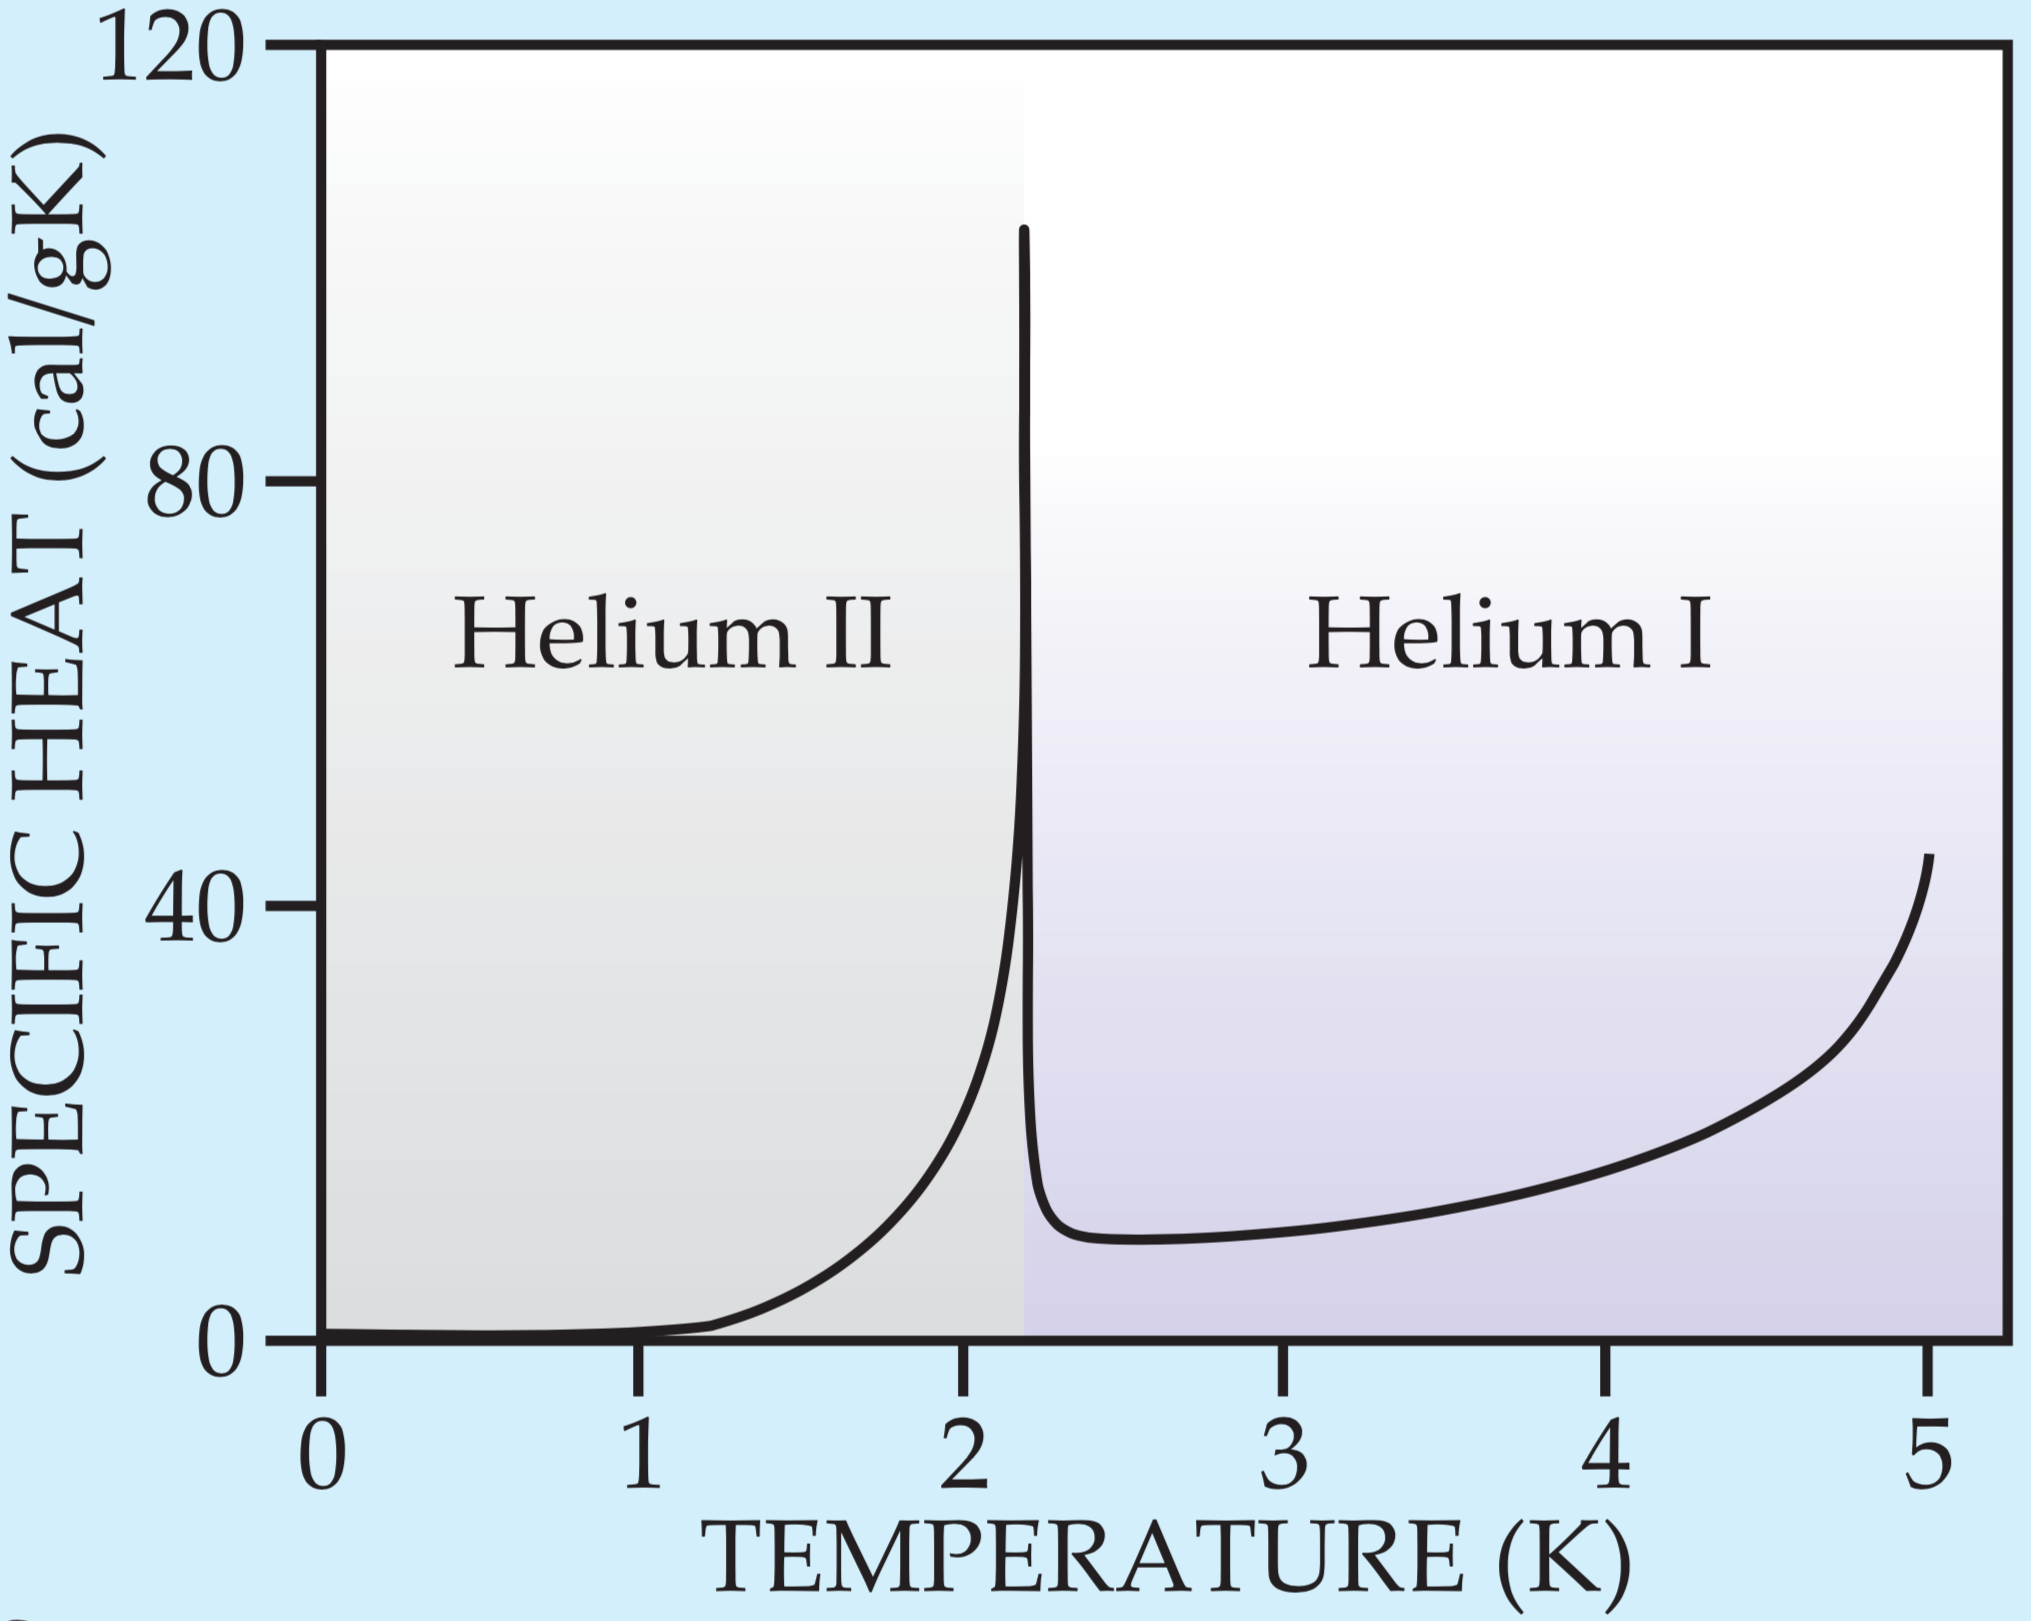
\includegraphics[width=0.75\textwidth]{specific-heat}
		\end{center}
		\caption{The specific heat of $^4$He as a function of the temperature. There is a clearly visible singularity around $2.2\unit{K}$ and the graph itself has the distinct $\lambda$-like shape that inspired Willem and Anna Keesom to call the temperature at which the singularity occurs the ``$\lambda$-point''.}
		\label{fig:specific-heat}
	\end{figure}	
	
	\section{A brief history of superfluidity}
		\lettrine[lines=3,findent=3pt,nindent=0pt]{H}{elium} was the last gas to be liquefied and was done so by Kamerlingh Onnes in 1908[\emph{ref}]. In 1932 John McLennan saw[\emph{ref}] that liquid helium stopped boiling below $\approx\!2.2\unit{K}$ and later that year Willem Keesom and his daughter Anna observed[\emph{ref}], while measuring  the temperature dependence of the specific heat, a singularity around the same temperature. They called it the ``$\lambda$-temperature'',  $T_\lambda$, because of the shape of the temperature dependence of the specific heat resembling the Greek letter $\lambda$ (see Figure \ref{fig:specific-heat}). A few years later in 1935 Burton measured a sharp decrease in the viscosity of liquid helium below $T_\lambda$. Around the same time Fritz London was already thinking about macroscopic wave functions and why helium does not freeze at $T=0\unit{K}$ under atmospheric pressure. He concluded that it was caused by the zero point motion of the helium atoms and their associated kinetic energy that is comparable to their Van der Waals energy, effectively preventing liquid helium to solidify. The year after, in 1936, Willem and Anna Keesom measured an abnormally high heat conductance below $T_\lambda$. This was confirmed roughly one year later by J.F. Allen \emph{et al.} and it was understood that the high thermal conductance was the reason for the helium to stop boiling whenever the temperature drops below $T_\lambda$. It was in 1937 when Kapitza tried to determine the viscosity of the laminar flow that he measured a viscosity that was about $10^4$ times smaller than that of hydrogen gas. It was then that Kaptiza who, by analogy with superconductors, first coined the word ``superfluid'' to describe the special state that helium enters below the $\lambda$-point where it can flow, seemingly without friction. Allen and Misner realised that superfluid helium is not just a liquid with a very low viscosity, but that its hydrodynamics was completely different from that of ordinary liquids and therefore required a completely new interpretation.\\
		
		The start of this new interpretation was made by London in 1938 when he made a connection between the behaviour of superfluid helium and that of an ideal Bose-Einstein (BE) gas. Both his calculated value for $T_c=3.09\unit{K}$ and the behaviour of the temperature dependence of the heat capacity for the ideal BE-gas were very similar to the measured ones for liquid helium below $T_\lambda$. He wrote to Nature that ``it was difficult not to imagine a connection with Bose-Einstein condensation'' (BEC). Laszlo Tisza expanded upon London's ideas and considered a Helium II system of total $N$ atoms to consist of two parts; a macroscopic ``condensed'' part $n_0$, the superfluid component, in the ground state, and the remaining part $n=N-n_0$, the normal component, where the helium atoms are distributed over the excited states. Assuming this was correct the fraction $n_0/N$ should decrease with increasing temperature according to the equation\\
		\begin{align}
			\frac{n_0}{N} = 1-\qty(\frac{T}{T_0})^s \quad \text{for} \quad T<T_0
		\end{align}
		where $s=3/2$ for an ideal gas and should be taken larger, e.g. $s=5$, for a real liquid with stronger interactions between the atoms.\\
		
		This was the birth of the ``two-fluid'' model. With this model he derived two hydrodynamic equations for liquid helium below $T_\lambda$ and discovered that within it, heat propagates in waves instead of diffusing through the medium, and calculated the velocity of these waves. He also explained why the viscosity is disappearing at low temperatures [\emph{this is explained in the french paper I still have to read}] contrary to classical liquids where the viscosity increases. In 1941 Lev Landau reformulated Tisza's theory on a more rigorous footing. He assumed, contrary to Tisza, that the normal component of the liquid was made-up of collective excitations instead of excited single atoms. He postulated that the liquid could exhibit two states of motion which he called ``potential motion'' that is irrotational ($\curl{\vec{v}}=0$), and ``vortex motion'' that is rotational ($\curl{\vec{v}} \neq 0$). The corresponding energies of these two motions are discontinuously separated by an energy gap $\Delta$. In case of potential internal motion  the excitations are quanta of longitudinal (sound) waves, i.e., phonons. The excitations of the vortex-spectrum could be called ``rotons''(see Figure \ref{fig:phonon-roton}).\\

		\begin{figure}[t]
			\begin{center}
				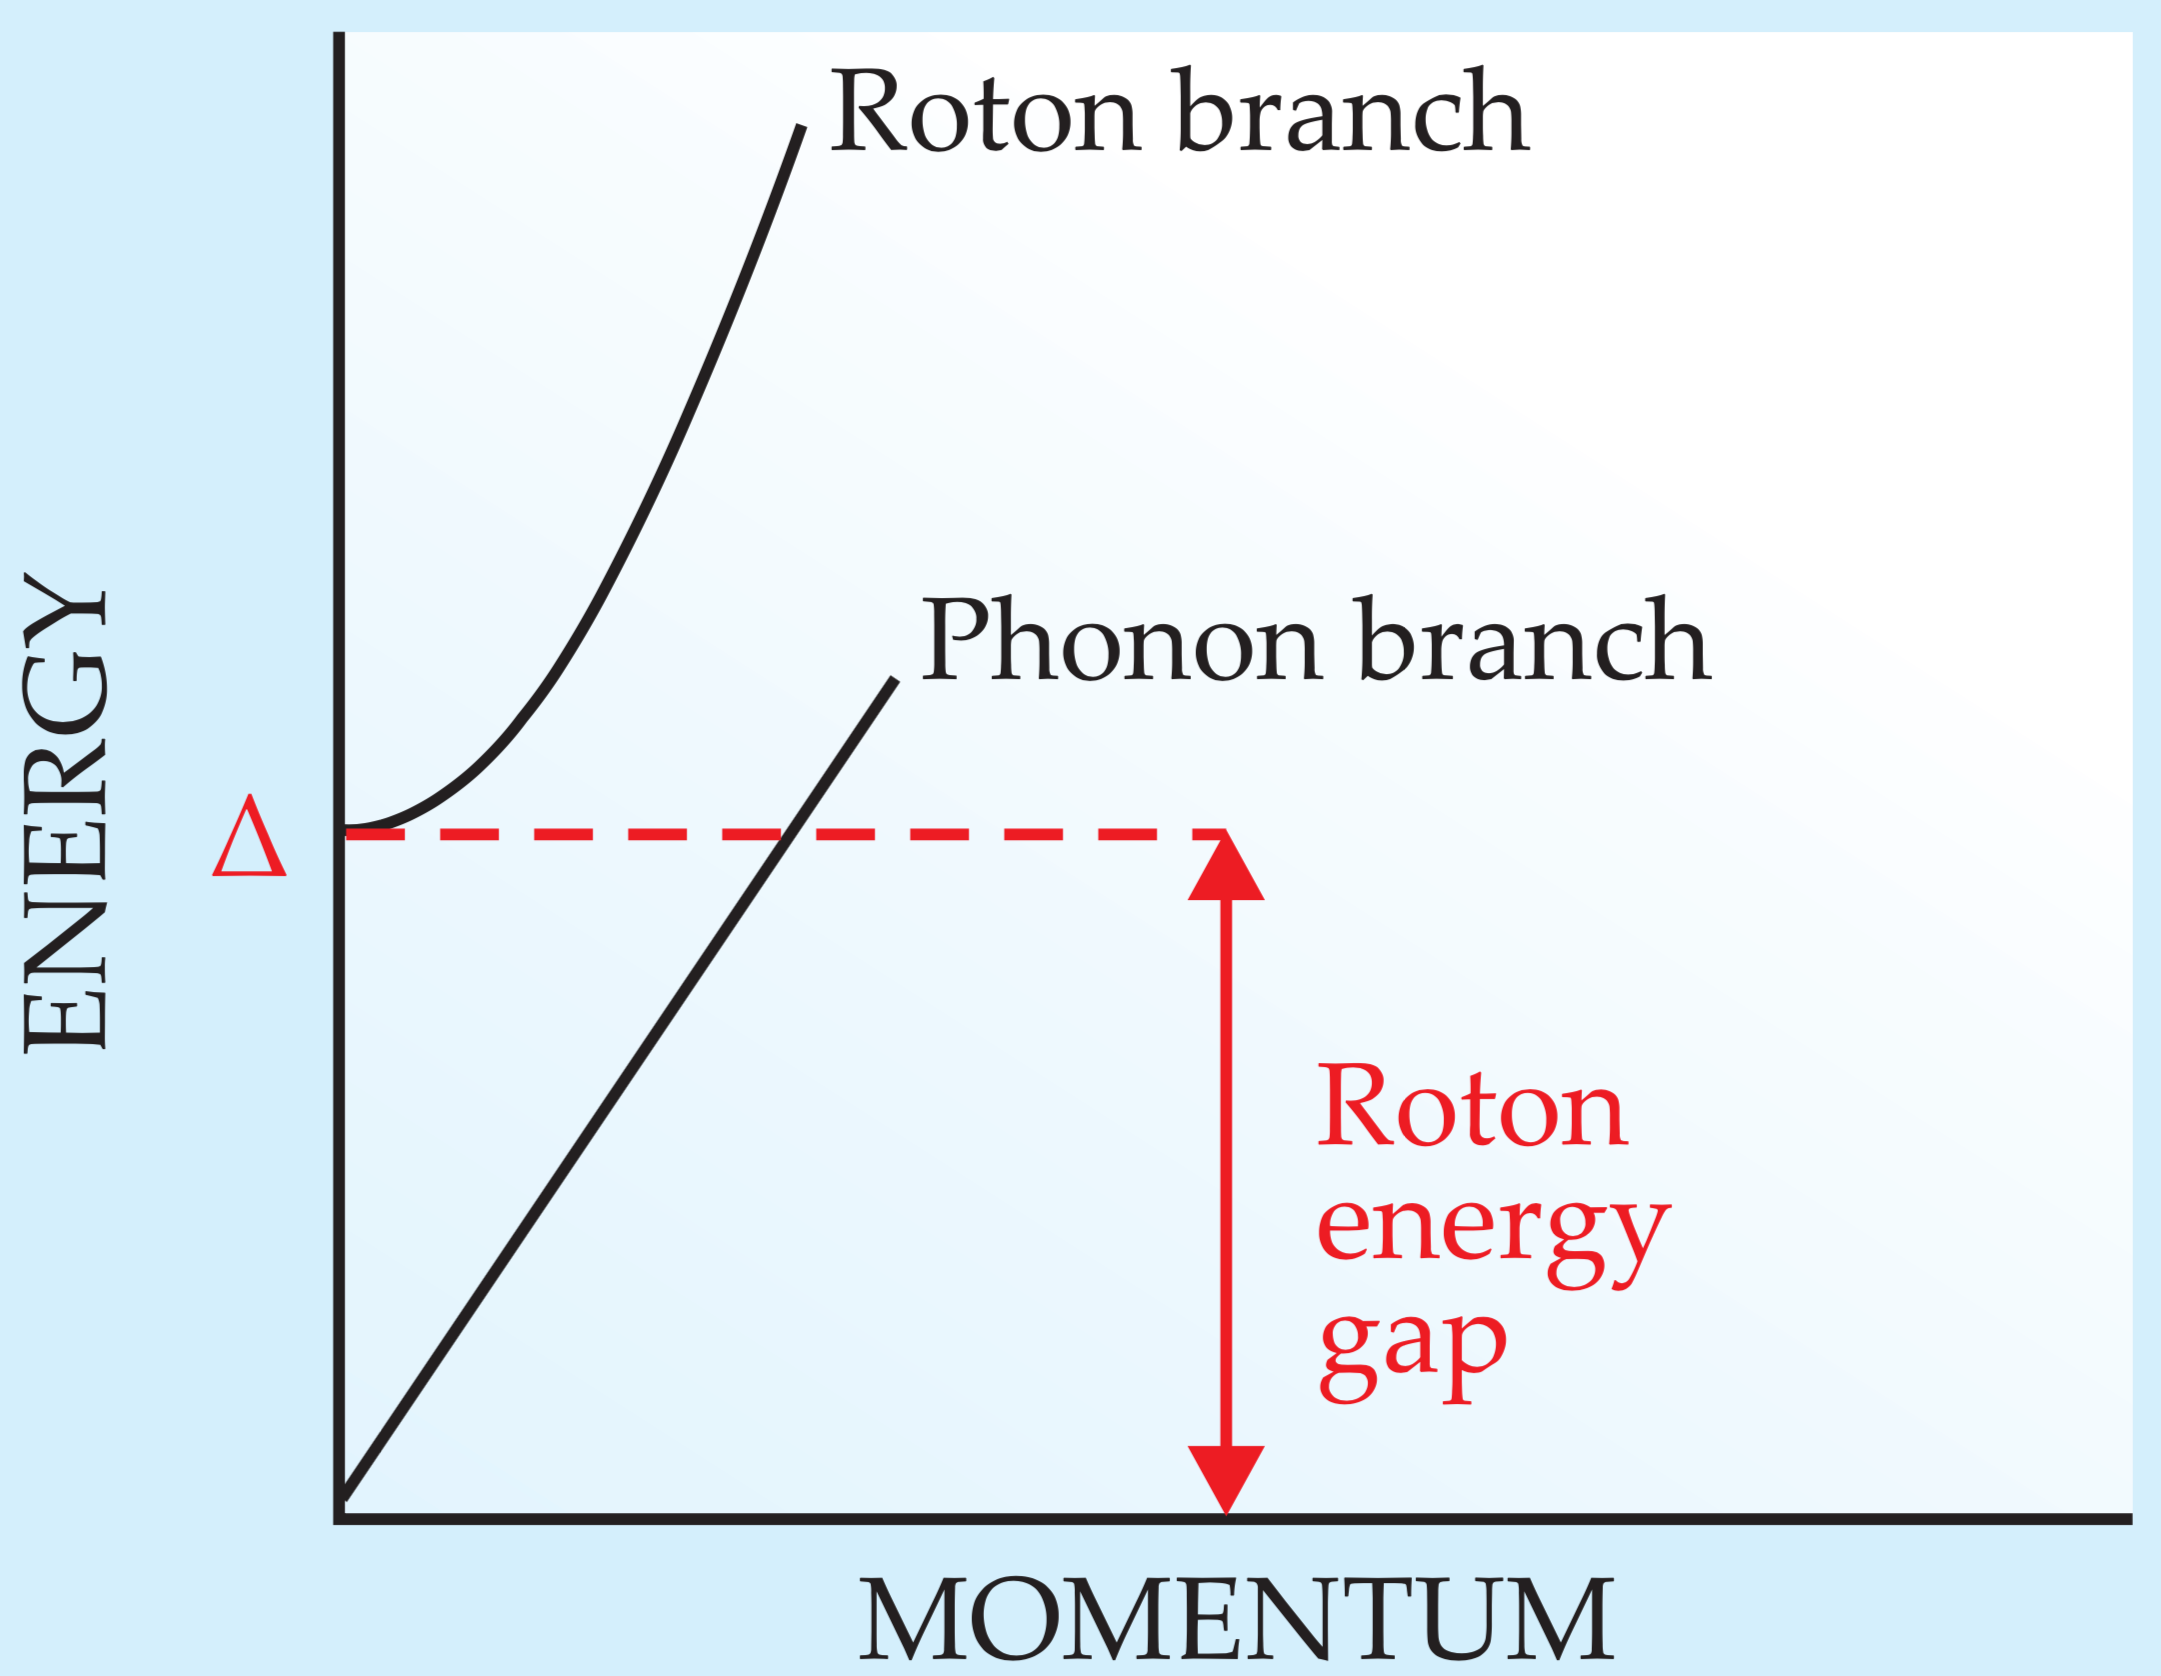
\includegraphics[width=0.495\textwidth]{phonon-roton-landau-first}
				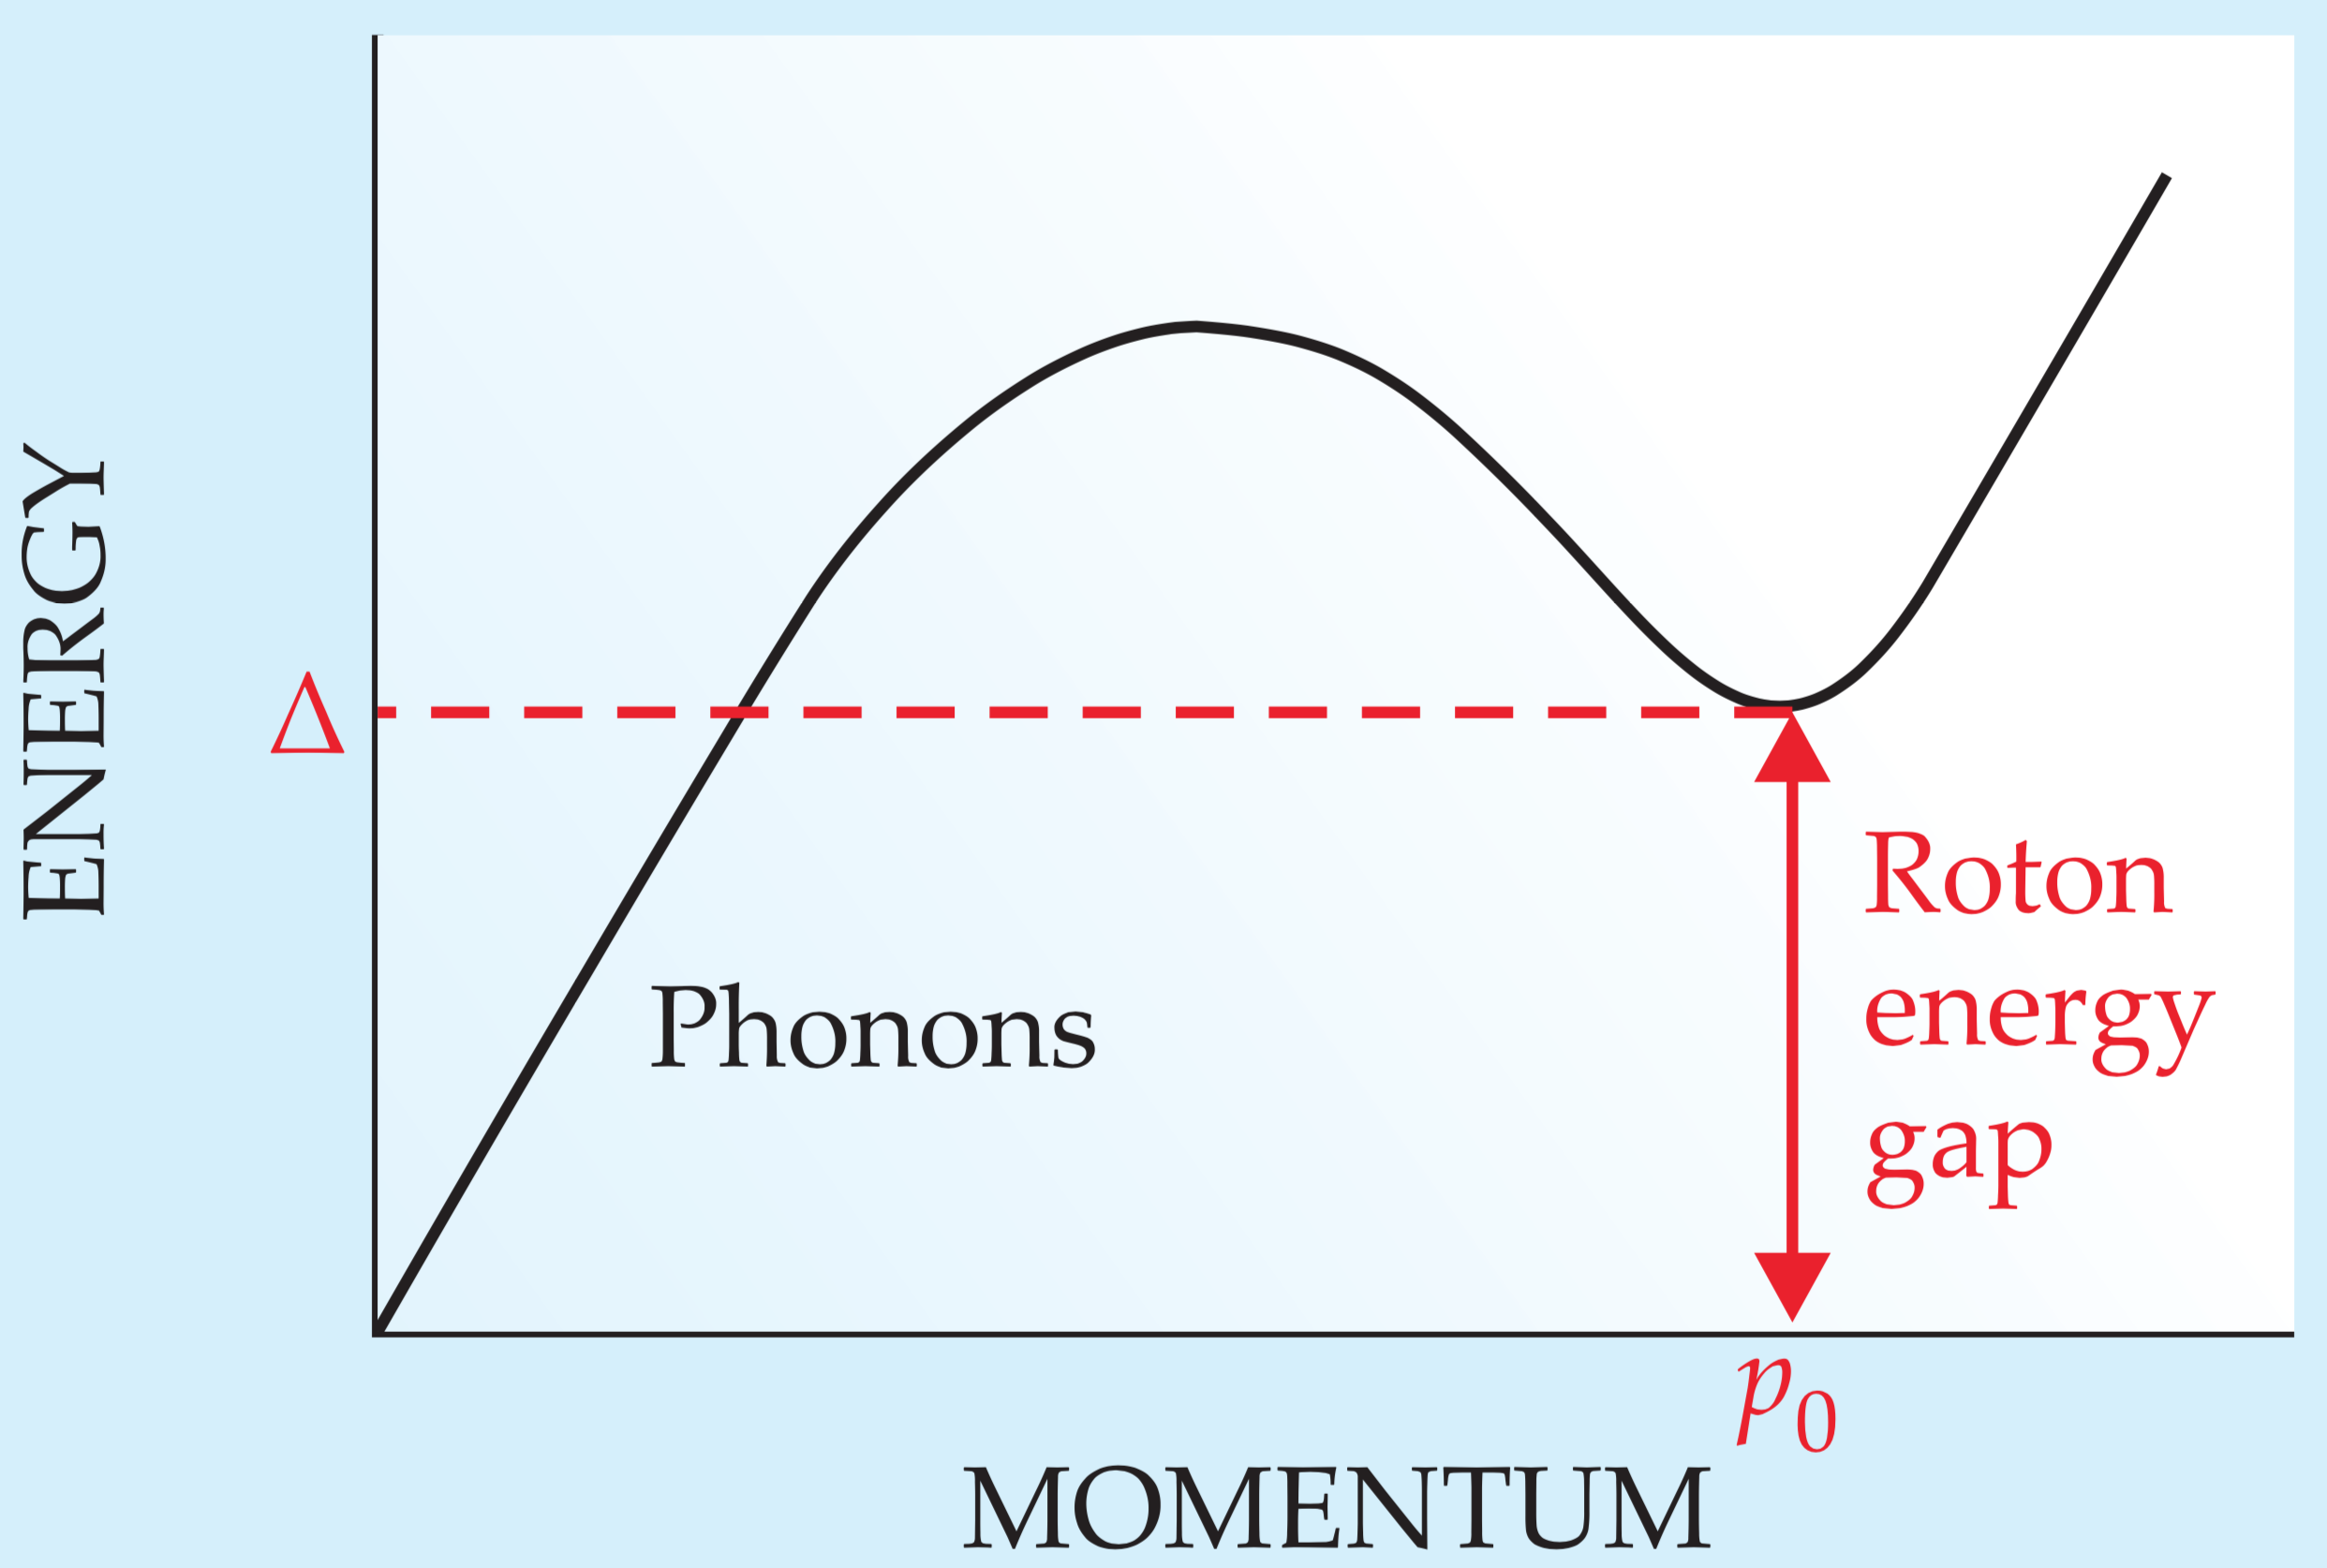
\includegraphics[width=0.495\textwidth]{phonon-roton-bogoliubov}
			\end{center}
			\caption{Left: Lev Landau's 1941 energy dispersion curve for the excitations in liquid helium below $T_\lambda$. It exhibits a phonon- and a roton branch. The slope of the linear phonon branch corresponds to the velocity of sound. Right: Lev Landau's (Bogoliubov's) 1947 corrected dispersion curve. The roton-branch is no longer a separate excitation branch but rather an extension of the phonon-branch.}
			\label{fig:phonon-roton}
		\end{figure}

		A theoretical demonstration, explicitly showing that phonons and rotons are collective excitations of the liquid, came in the form of a 1947 paper by Nikolay Bogolyubov[ref]. The intimate relationship between superfluidity and BEC was not universally accepted until 1995 when Cornell and Wienman in Colorado and Ketterle at MIT discovered BEC in rubidium quantum gases[ref].

	\section{Some key concepts}
		\lettrine[lines=3,findent=3pt,nindent=0pt]{I}{n} this section I will briefly introduce some key ideas that are used throughout the thesis and that are needed to fully appreciate the discussed material. Also references to more complete and more in-depth treatments will be provided for the interested reader.
		
		\subsection{Bose-Einstein condensation and long-range order}
			The essential concept of Bose-Einstein condensation is the fact that at low temperatures, multiple bosons, unlike fermions, will occupy the same quantum state. In theory there is no upper bound of how many bosons can occupy such a single state. It is then said that, with ever decreasing temperature, a macroscopic part of the total number of bosons will ``condense'' into the quantum state with the lowest energy.\\			
			
			Another important concept in BEC is the idea of long-range order. Let us start by introducing the one-body density matrix of a system of $N$ bosons in a pure state $\Psi_k(\vec{r}_1,\vec{r}_2,\ldots,\vec{r}_N)$
			\begin{align}
				n^{(1)}_k(\vec{r},\vec{r'}) \vcentcolon= N\int\!	\Psi_k^*(\vec{r},\vec{r}_2,\ldots,\vec{r}_N)\Psi_k(\vec{r'},\vec{r}_2,\ldots,\vec{r}_N)\diff{r}_2\diff{r}_3\ldots\diff{r}_N	\label{eq:def-obd-matrix}
			\end{align}
			where the integral is taken over the $N-1$ coordinates $\vec{r}_2,\vec{r}_3,\ldots,\vec{r}_N$. For a statistical mixture of quantum states one needs to take the weighted average over all the different $\Psi_k$-states. In thermodynamic equilibrium the states are Boltzmann weighted by their eigenvalues $\qty{E_k}$
			\begin{align}
				n^{(1)}(\vec{r},\vec{r'}) = \frac{1}{Q}\sum_k n^{(1)}_k(\vec{r},\vec{r'}) \unit{e}^{-E_k/k_BT}
			\end{align}
			where $Q$ is the partition function. For more general cases the one-body density matrix is defined
			\begin{align}
				n^{(1)}(\vec{r},\vec{r'}) \vcentcolon=\expval{\hat\Psi^\dagger(\vec{r})\hat\Psi(\vec{r'})}
			\end{align}
			where $\hat\Psi^\dagger(\vec{r})$/$\hat\Psi(\vec{r})$ are field-operators creating/annihilating a boson at $\vec{r}$ and the averaging $\expval{\cdots}$ is taken over all states in the mixture. Once it is accepted that a macroscopic part of the total number of bosons can occupy a single quantum state it can be demonstrated that, while considering a uniform isotropic sytem of $N$ bosons, the one-body density matrix (Eq. \ref{eq:def-obd-matrix}) tends to a constant value when the distance between $\vec{r}$ and $\vec{r}'$ goes to infinity. In the thermodynamic limit where $N,V\rightarrow\infty$ such that $n=N/V$ is kept fixed, the one-body density only depends on the modulus of the relative variable $\vec{s}:=\vec{r}-\vec{r}'$ so that we can write it as the Fourier transform of the momentum distribution as
			\begin{align}
				n^{(1)}(s) = \frac{1}{V}\int \! n^{(1)}\qty(\vec{p})\exp(i\vec{p}\cdot\vec{s}/\hbar)\,\mathrm{d}\vec{p} \label{eq:one-body-den-mom}
			\end{align}
			For a Bose-Einstein condensed system, the momentum distribution at small momenta is not smooth but has a sharp peak around $p=0$ for the bosons that are in the ground state, while the remaining bosons are smoothly distributed over the excited states.
			\begin{align}
				n(\vec{p})=N_0\delta(\vec{p})+\tilde{n}(\vec{p})
			\end{align}
			where $\tilde{n}$ is a smoothly varying function of $\vec{p}$. When this expression is plugged into Eq. (\ref{eq:one-body-den-mom}) and taking the limit where $s$ goes to infinity
			\begin{align}
				\lim_{s\rightarrow\infty}n^{(1)}(s)=\frac{N_0}{V},
			\end{align}
			where $N_0/V \vcentcolon= n_0\leq 1$ is called the condensate fraction. It is called long-range order since it involves the off-diagonal elements of the one-body density matrix; the elements that are usually associated with the coherences.\\
			
			A set of eigenvalues \{$n_i$\} of the one-body density matrix can be defined through the following eigenvalue equation
			\begin{align}
				\int \! n^{(1)}(\vec{r},\vec{r'})\varphi_i(\vec{r'}) \,\mathrm{d}\vec{r'} = n_i\varphi_i(\vec{r})
			\end{align}
			and its solutions \{$\varphi_i$\} form a natural orthonormal basis set of single boson wave functions $\int\!\varphi_i^*\varphi_j\,\mathrm{d}\vec{r}=\delta_{ij}$, with normalisation condition $\sum_i n_i=N$. This permits writing the on-body density matrix in a useful diagonalised form and recalling that Bose-Einstein condensation occurs when a single particle state $\varphi_i$ is occupied in a macroscopic way, say when $n_{i=0}=N_0$, a number of order $N$, we separate the condensate part from the rest
			\begin{align}
				n^{(1)}(\vec{r},\vec{r'}) = N_0\varphi_0^*(\vec{r})\varphi_0(\vec{r'})+\sum_{i\neq0}n_i\varphi_i^*(\vec{r})\varphi_i(\vec{r'}) \label{eq:obdm-diag}
			\end{align}

		\subsection{Bogolyubov's approximation and the order parameter}\label{sec:bogol-order}
			It is customary, given the importance of the condensate fraction $N_0$ in a BEC, to write the field operator of a $N$-body boson system as the sum of the condensate part and the rest, just as the one-body density matrix
			\begin{align}
				\hat{\Psi}(\vec{r})=\varphi_0(\vec{r})\hat{a}_0 + \sum_{i\neq 0} \varphi_i(\vec{r})\hat{a}_i \label{eq:field-operator}
			\end{align}
			where the $\hat{a}_i$ and $\hat{a}_i^\dagger$ are annihilation and creation operator of a particle in state $\varphi_i$ and obey the usual bosonic commutation relations
			\begin{align}
				\commutator{\hat{a}_i}{\hat{a}_j^\dagger}=\delta_{ij},\quad 	\commutator{\hat{a}_i}{\hat{a}_j}=0=\commutator{\hat{a}_i^\dagger}{\hat{a}_j^\dagger}
			\end{align}
			Using Eq. (\ref{eq:field-operator}) in Eq. (\ref{eq:def-obd-matrix}) and comparing it to Eq. (\ref{eq:obdm-diag}) one finds the expectation value of $\expectationvalue{\hat{a}_j^\dagger\,\hat{a}_i}=\delta_{ij}n_i$. Now, the Bogolyubov approximation essentially replaces the operators $\hat{a}_0$ and $\hat{a}_0^\dagger$ with the $c$-number\footnote{The term $c$-number is old nomenclature for a classical number, which can be real or complex, to distinguish them from quantum numbers, or $q$-numbers, that are represented by operators.} $\sqrt{N_0}$. This is equivalent to ignoring the non-commutative nature of the operators due to the macroscopic occupation of the state $\varphi_0$, when $N_0=\expectationvalue{\hat{a}_0^\dagger\,\hat{a}_0}\gg 1$. We then rewrite the field operator as the sum of a classical field for the condensed component and quantum field for the non-condensed component
			\begin{align}
				\hat{\Psi}(\vec{r})=\Psi_0(\vec{r})+\delta\hat{\Psi}(\vec{r}),\label{eq:order-param-real}
			\end{align}
			where $\delta\hat{\Psi}(\vec{r})=\sum_{i\neq 0}\varphi_i(\vec{r})\hat{a}_i$ and $\Psi_0(\vec{r})=\sqrt{N_0}\varphi_0(\vec{r})$. At $T=0$ the whole system is condensed and one can ignore $\delta\hat{\Psi}$ altogether; the field operator becomes a normal function of space $\Psi_0$.\\
			
			The classical field $\Psi_0$ is called the \emph{effective}- or \emph{macroscopic} wave function of the condensate and it behaves like an order parameter in the sense that it varies continuously between a maximum value $\sqrt{N}$, that is proportional to the total number particles in the system, at $T=0$, and vanishes at the superfluid-normal fluid phase transition temperature $T_\lambda$. It is a complex quantity characterised by a real-valued modulus and phase $S$:
			\begin{align}
				\Psi_0(\vec{r}) = \absolutevalue{\sqrt{N_0}\varphi_0(\vec{r)}}\,\mathrm{e}^{iS(\vec{r})}\label{eq:order-param-complex}
			\end{align}
			The modulus determines the number-density of the condensate, while the phase $S$ plays an important role in the coherence and properties of the superfluid. As we will see in Section \ref{sec:rot-vort}, $S$ plays the role of a velocity potential.\\
			
			Using an order parameter as defined here is equivalent to using the many-body wave function
			\begin{align}
				\Phi(\vec{r}_1,\vec{r}_2,\ldots\vec{r}_N)=\prod_{i=1}^{N}\varphi_0(\vec{r}_i),
			\end{align}
			with a density operator $\hat{\rho}(\vec{r}) \vcentcolon= \sum_{i=1}^{N}\delta(\vec{r}-\vec{r}_i)$ (see Section \ref{sec:dft-method}). One way to see why this wave function plays the role of an order parameter is to look at its time dependence. For normal wave functions the time dependence is determined by the eigenvalues $E_i$ of the Hamiltonian of the system
			\begin{align}
				\Psi(\vec{r},t)=\psi(\vec{r})\,\mathrm{e}^{-iE_it/\hbar}
			\end{align}
			But in this case, the time dependence is determined by the chemical potential $\mu=E(N)-E(N-1)\approx \partial E/\partial N$
			\begin{align}
				\Psi_0(\vec{r},t)=\Psi_0(\vec{r})\,\mathrm{e}^{-i\mu t/\hbar} \label{eq:td-order-param}
			\end{align}
			Another aspect of $\Psi_0$ being an order parameter and not a true many-body wave function is that two solutions $\Psi_a$ and $\Psi_b$ of the non-linear droplet Hamiltonian corresponding to two different values of the chemical potential $\mu_a$ and $\mu_b$ are not necessarily orthogonal, i.e. $0 \leq N^{-1}\int\!\Psi_a^*\Psi_b\unit{d}\vec{r} < 1$. However, in dilute gases it is possible to construct a many-body wave function from the order parameter that regains its orthonormality in the thermodynamic limit
			\begin{align}
				\Phi_0(\vec{r}_1,\vec{r}_2,\ldots,\vec{r}_N) = \qty(\frac{1}{\sqrt{N}}\Psi_0(\vec{r}_1))\qty(\frac{1}{\sqrt{N}}\Psi_0(\vec{r}_2))\cdots\qty(\frac{1}{\sqrt{N}}\Psi_0(\vec{r}_N))
			\end{align}
			
		\subsection{Landau's criterion for superfluidity}
			\begin{figure}[t]
				\begin{center}
					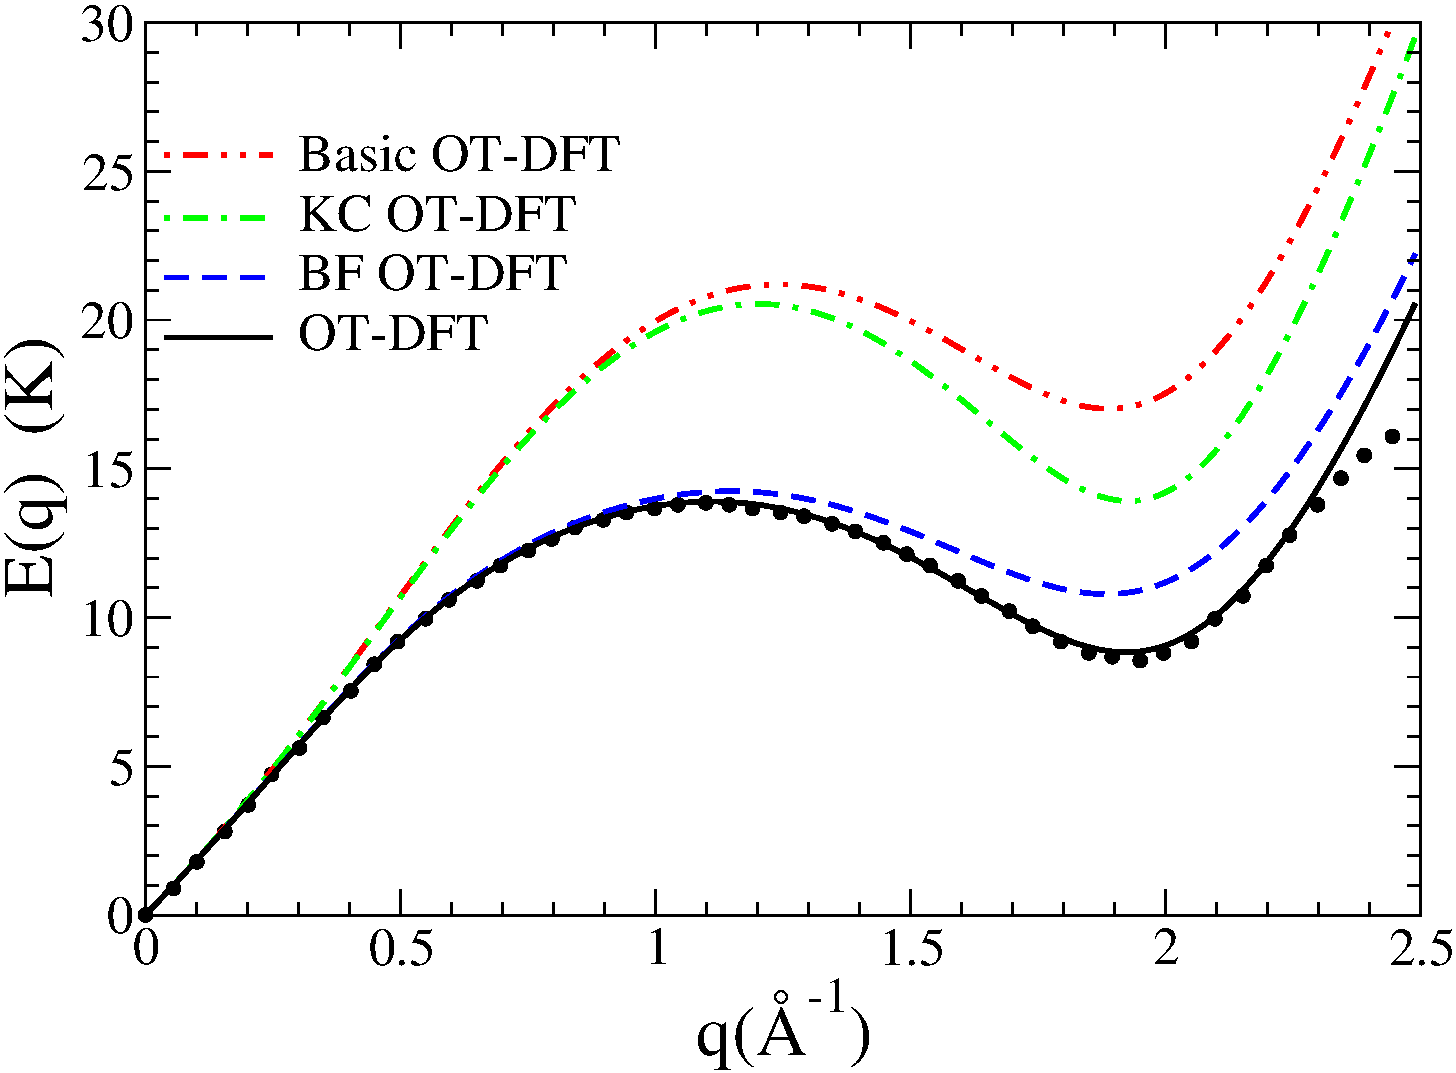
\includegraphics[width=0.9\textwidth]{dispersion-relation}
					\caption{Dispersion relation for elementary excitations in liquid $^4$He calculated as in  \cite{Mat10a}. `Basic' indicates the OT-DFT without the non-local kinetic energy correlation (KC) nor the back-flow (BF) terms; KC OT-DFT adds  to the basic OT-DFT the KC term; BF OT-DFT adds to the basic OT-DFT the BF term. The dots are the experimental data from \cite{Don81}. The Landau velocity $v_L = E(q)/(\hbar\,q)|_{min}$ obtained for each functional is  60.3 m/s (OT-DFT); 75.1 m/s (BF OT-DFT); 94.4 m/s (KC OT-DFT); 118 m/s (basic OT-DFT); and 57.5 (experiment).}
					\label{fig:dispersion-relation}
				\end{center}
			\end{figure}
		
			For a gas or liquid to be able to become superfluid Landau postulated that the energy dispersion relation needs to fulfil certain requirements. Specifically for a fluid to flow  without dissipation, i.e. a super-flow, the velocity field needs to fulfil the following inequality:
			\begin{align}
				v<v_c = \min_{\vec{p}}\frac{\epsilon(\vec{p})}{p}
			\end{align}
			
			For an ideal Bose gas $\epsilon(\vec{p})= \frac{p^2}{2m}$. In this case 
			\begin{align}
				v_c &= \min_{\vec{p}}\frac{\epsilon(\vec{p})}{p} \\
					&= \min_{\vec{p}}\frac{p}{2m} \\
					&= 0
			\end{align}
			Apparently ideal Bose-gases cannot become superfluid.\\
			
			But if we allow for some weak interactions between the bosons the energy dispersion relation is given by
			\begin{align}
				\epsilon(\vec{p})=\sqrt{\frac{gn}{m}p^2+\qty(\frac{p^2}{2m})^2},
			\end{align}
			Bogolyubov's dispersion law for elementary excitations (1947). And thus
			\begin{align}
				v_c &=\min_{\vec{p}}\sqrt{\frac{gn}{m}+\frac{p^2}{4m^2}} \\
					&= \sqrt{\frac{gn}{m}} \\
					&= c,
			\end{align}
			the speed of sound. Here $g=\frac{4\pi\hbar^2a}{m}$, and $a$ the $s$-wave scattering length. The weakly interacting Bose gases can become superfluid.\\			

			Liquid helium below the $\lambda$-point has a similar energy dispersion relation (see Figure \ref{fig:dispersion-relation}) hence reinforcing the notion that superfluidity and Bose--Einstein condensation are two intimately related concepts. The experimental value of the speed of sound is $\sim\!57.5\unit{m/s}$.
			
		\subsection{Rotation and vorticity in superfluids}\label{sec:rot-vort}
			\begin{figure}[t]
				\begin{center}
					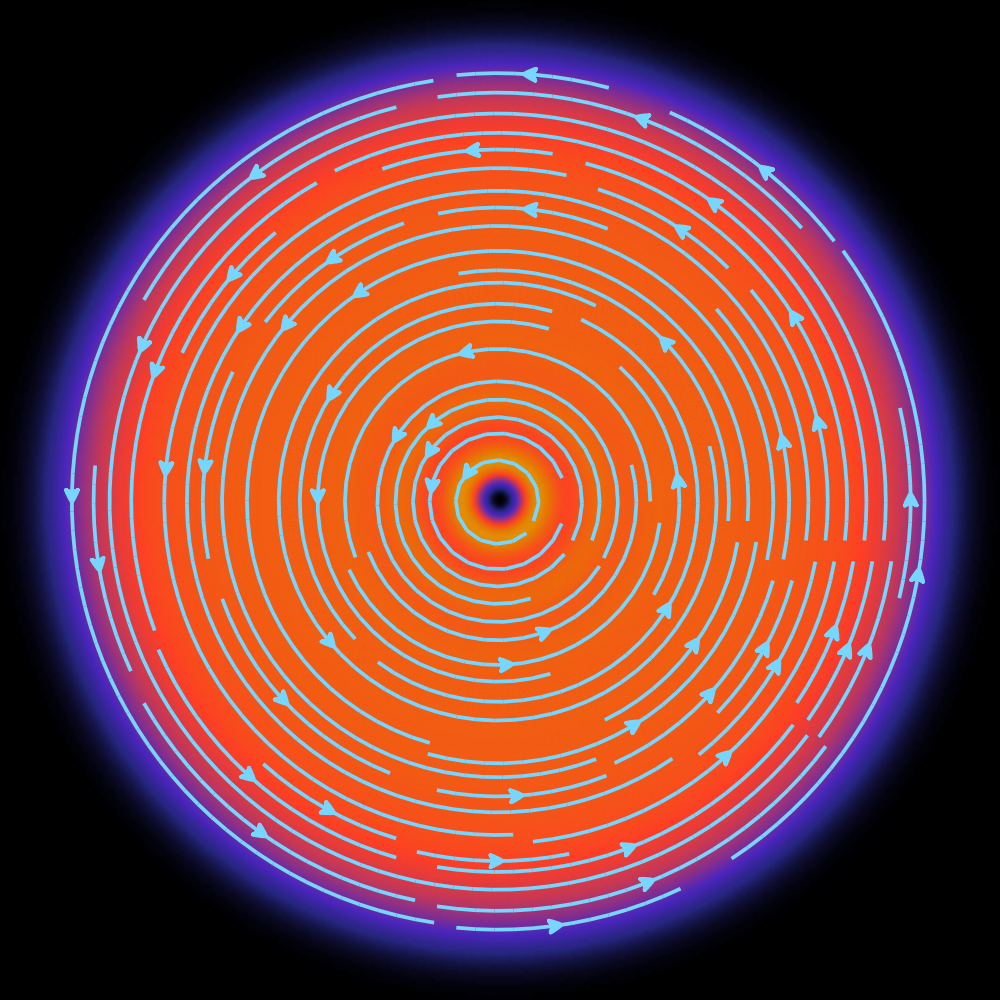
\includegraphics[width=0.5\textwidth]{vortex-xy}
					\caption{Cross section of a $^4$He droplet through a symmetry plane. The droplet is made of 1000 atoms. Superimposed in cyan are the streamlines of the velocity field $\vec{v}_s$ for $s=1$. They are concentric circles, centred around the vortex core along the $z$-axis. The colour scale encodes for the density $\rho(r)$. The radius of the droplet is about 22\,\AA.}
					\label{fig:vortex-xy}
				\end{center}
			\end{figure}
		
			Starting from time-dependent Euler--Lagrange (EL) equation (Eq. \ref{eq:td-el-equation}, see Chapter \ref{sec:dft-method}) for the time-evolution of the order parameter $\Psi$ (Eq. \ref{eq:order-param-complex}, dropping the ground-state subscript and allowing $\varphi$ and $S$ to vary in time)
			\begin{align}
				i\hbar\frac{\partial}{\partial t} \Psi({\mathbf r},t) = \left[-\frac{\hbar^2}{2m}\laplacian + \frac{\delta{\cal E}_{c}}{\delta\rho}\right]\Psi(\textbf{r},t)
			\end{align}
			one left-multiplies it with the complex conjugate of the order parameter $\Psi^*$ and then subtract the complex conjugate of the whole expression on both sides. After some algebra and defining $\rho(\vec{r},t)\vcentcolon=N\abs{\varphi(\vec{r},t)}^2$, one arrives at the continuity equation
			\begin{align}
				\frac{\partial\rho}{\partial t} + \div{\vec{j}}=0, \label{eq:continuity-eq}
			\end{align}
			with
			\begin{align}
				\vec{j}(\vec{r},t) \vcentcolon=& -\frac{i\hbar}{2m}\qty\Big[\Psi^*(\vec{r},t)\grad{\Psi}(\vec{r},t) - \Psi(\vec{r},t)\grad{\Psi^*}(\vec{r},t)] \\
					=&\,\rho(\vec{r},t)\frac{\hbar}{m}\grad{S(\vec{r},t)}
			\end{align}
			From Eq. (\ref{eq:continuity-eq}) it follows that the atomic number density is a conserved quantity (\textbf{HOW DOES THIS CORRELATE WITH EVAPORATION ?}).\\
			
			We can identify the collective velocity $\vec{v}_s$ of the superfluid through the relation
			\begin{align}
				\vec{v}_s(\vec{r},t) = \vec{j}/\rho=\frac{\hbar}{m}\grad{S(\vec{r},t)} \label{eq:velocity-field}
			\end{align}
			and we see that the rotation of the velocity field of the superfluid $\curl{\vec{v}_s}=0$, i.e. the fluid is said to be \emph{irrotational}; a typical property of superfluids. Conversely, taking the curl $\curl{\vec{j}}=\frac{\hbar}{m}\grad{\rho}\times\grad{S}$ we see that this is merely a restatement of the fact that one needs a gas or liquid with a non-uniform density and a non-zero phase for it to be able to support vortices.\\
			
			Let us consider the illustrative example of a line vortex through the origin along the $z$-axis. As will be demonstrated in Section \ref{sec:vortical-states}, this is a stationary state of the droplet Hamiltonian and therefore its time dependence is just a multiplicative factor. In cylindrical coordinates $(r,\varphi,z)$ such a vortex solution has the form
			\begin{align}
				\Psi_s(\vec{r}) = \sqrt{\rho(r)}\unit{e}^{is\varphi}, \label{eq:line-vortex}
			\end{align}
			with $s$ an integer. This is an eigenfunction of the angular momentum operator $\hat{L}_z$ with eigenvalue
			\begin{align}
				\hat{L}_z \Psi_s(\vec{r}) &= \frac{\hbar}{i}\frac{\partial}{\partial\varphi}\Psi_s(\vec{r}) = \hbar s\Psi_s(\vec{r})
			\end{align}
			and with expectation value
			\begin{align}
				\expval{\hat{L}_z} &= \expval{\hat{L}_z}{\Psi_s} \\
					&= \hbar s \braket{\sqrt{N_0}\varphi_0} \\
					&= N_0\hbar s
			\end{align}
			The angular momentum is quantised and proportional to the number of bosons in the BEC fraction/superfluid. We can calculate the velocity field
			\begin{align}
				\vec{v}_s = \frac{\hbar}{m}\grad{S} = \frac{\hbar}{m}\frac{s}{r}\,\vu*{\varphi}
			\end{align}
			The streamlines of $\vec{v}_s$ are concentric circles, centred around the z-axis, lying in the $xy$-plane (see Figure \ref{fig:vortex-xy}). Contrary to rigid rotation fields which increase proportional to the distance from the $z$-axis $r$, the superfluid rotation field decreases proportional to distance from the $z$-axis $1/r$ and is singular in the origin. Calculating the circulation of the velocity field $\vec{v}_s$ along a closed contour including the $z$-axis gives
			\begin{align}
				\oint_{\partial\Sigma}\!\vec{v}_s\cdot\unit{d}\vec{l} &=
				\int_{0}^{2\pi}\!\frac{\hbar}{m}\frac{s}{r}\,\vu*{\varphi}\cdot r\unit{d}\varphi\,\vu*{\varphi} \\
					&= 2\pi s\frac{\hbar}{m}
			\end{align}
			There are two things to note here. Firstly, the circulation around a closed loop that encompasses the $z$-axis is quantised in units of $\hbar/m$ for $s\in\mathbb{N}_{>0}$. Secondly, the value of the circulation of the velocity field does not depend on the chosen contour as long as it includes the location of the vortex. This means that all the vorticity is contained at the location where the velocity field is singular (the ``core'' of the vortex), at $r=0$ along the $z$-axis.\\
			
			Because of the pole in the velocity field, Stokes theorem will lead to the following contradiction
			\begin{align}
				2\pi s\frac{\hbar}{m}=\oint_{\partial\Sigma}\!\!\!\vec{v}_s\cdot\unit{d}\vec{l} = \iint_{\Sigma}\!\curl{\vec{v}_s}\cdot\unit{d}\vec{\Sigma} = 0
			\end{align}
			and can therefore not be applied. To emphasise that all the vorticity is concentrated around the vortex core one can write formally
			\begin{align}
				\curl{\vec{v}_s} = 2\pi s\frac{\hbar}{m}\delta^{(2)}(\vec{r}_\perp)\,\vu{z},
			\end{align}
			where $\delta^{(2)}$ is 2-dimensional Dirac-delta function and $\vec{r}_\perp$ a vector in a plane perpendicular to the vortex line.\\

	\section{Helium droplets}
		\lettrine[lines=3,findent=3pt,nindent=0pt]{U}{ntil} the 1980, most experimental and theoretical work was done on bulk systems, i.e. systems of the order of $N_A$ number of atoms. It was only in the last couple of decades that advancements in technology enabled experimentalists to create nanoscale sized superfluid helium droplets. From the early 1990's onwards, superfluid helium nano-droplets became an active field of study, both experimentally and theoretically. Surely, the finite size of these droplets would impose some interesting properties as compared to bulk liquid helium.\\
		
		The helium-helium interaction is already weak in bulk liquid helium and in finite self-bound systems such as droplets it is even weaker, e.g. the binding energy per atom is $<\!7.17\unit{K}$. Because of this, helium droplets cool down very rapidly due to evaporation, reaching their limiting temperature of about $0.38\unit{K}$ in microseconds. Pure helium droplets are neutral systems and their properties like their size, binding energy and excitation spectra, are not easy to determine experimentally and are usually obtained by indirect methods. This didn't stop the theoreticians describe doped $^4$He$_N$ droplets using a wide variety of approaches depending on the size and character of the droplets ranging from Quantum Monte Carlo, Hypernetted-Chain/Euler-Lagrange, Variational Monte Carlo and many others.\\
	
		A key property of helium droplets, in contrast to bulk helium, is their ability to pickup any kind of dopants with which they collide. Depending on the relative strength of the He-dopant interaction compared to the He-He interaction, impurities either get bound to the surface of the droplet (e.g. the alkalies) or get absorbed into their interior. They can therefore be doped with almost any kind of atomic or molecular species where they can form new complexes. This enables a broad spectrum of possible experimental study. Due to the fact that helium droplet are ultra cold superfluid liquids, and therefore provide high mobility of any picked-up dopants, one can do high resolution spectroscopy studies. Having a fine control over the number of picked-up dopants[29] one can use droplets as a matrix for creating self-organising structures of polar molecules, or very cold metal clusters and study their Coulomb explosion. From the perspective of the droplet it's possible to use the dopants as gentle probes to determine the superfluid properties of helium droplets that would be inaccessible with other methods. For two examples of this see [37-39], where a dopant is used to probe the superfluid character of small $^4$He droplets and [16,17] to see their limiting temperatures.\\
		
		\begin{figure}[t]
			\begin{center}
				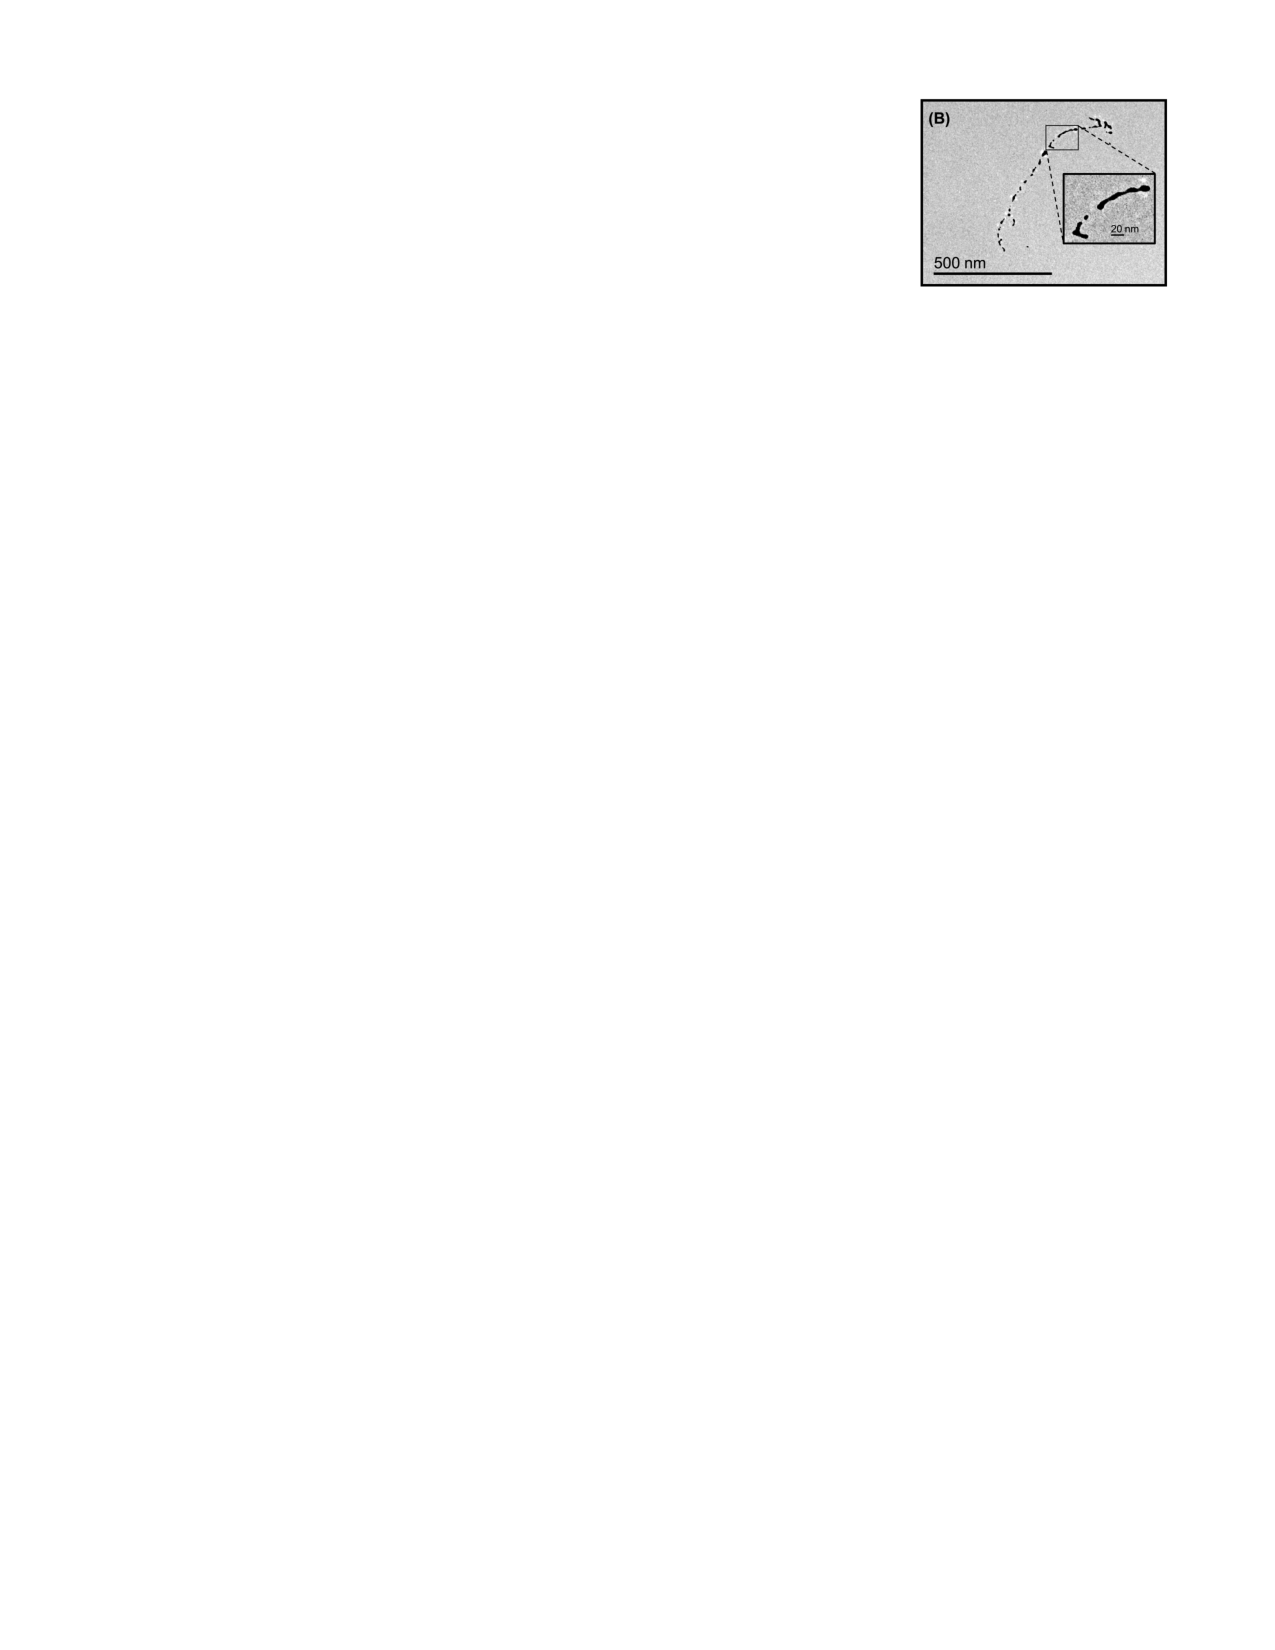
\includegraphics[width=0.75\textwidth]{silver-filament}
				\caption{Electron-microscope image of and elongated track-shaped Ag-cluster after it is surface-deposited.}
				\label{fig:silver-filament}
			\end{center}
		\end{figure}	
				
		One of the most intriguing properties of superfluid helium droplets is the fact that they can host quantised vortices. Because of their ultra low temperature they are true quantum liquids and thus their vorticity and angular momentum are quantised. The existence of quantised vortices was anticipated because they have been created and observed in Bose-Einstein condensates made of dilute gases. However, the detection of quantised vortices is still experimentally challenging. Recently, Gomez, Loginov and Vilesov performed experiments[PRL 108, 155302 (2012)] where vortices inside superfluid $^4$He droplets, produced by the expansion of liquid helium, were traced by introducing Ag atoms which clustered along the vortex lines, into the droplets. The Ag clusters were subsequently surface-deposited and imaged via electron microscopy. The prevalence of elongated track-shaped deposits (see Figure \ref{fig:vortex-array}) shows that vortices are present in droplets larger than about $300\unit{nm}$ and that their lifetime exceeds a few milliseconds. Two years later Gomez reported[Science 345, 906 (2014)] on the formation of quantum vortex lattices inside droplets. He used single-shot femtosecond x-ray coherent diffractive imaging to investigate the rotation of single, isolated superfluid helium-4 droplets containing $\sim\!10^8$ to $10^{11}$ atoms. The formation of quantum vortex lattices inside the droplets was confirmed by observing the characteristic Bragg patterns from xenon clusters trapped in the vortex cores (see Figure \ref{fig:vortex-array}).\\

		\begin{figure}[t]
			\begin{center}
				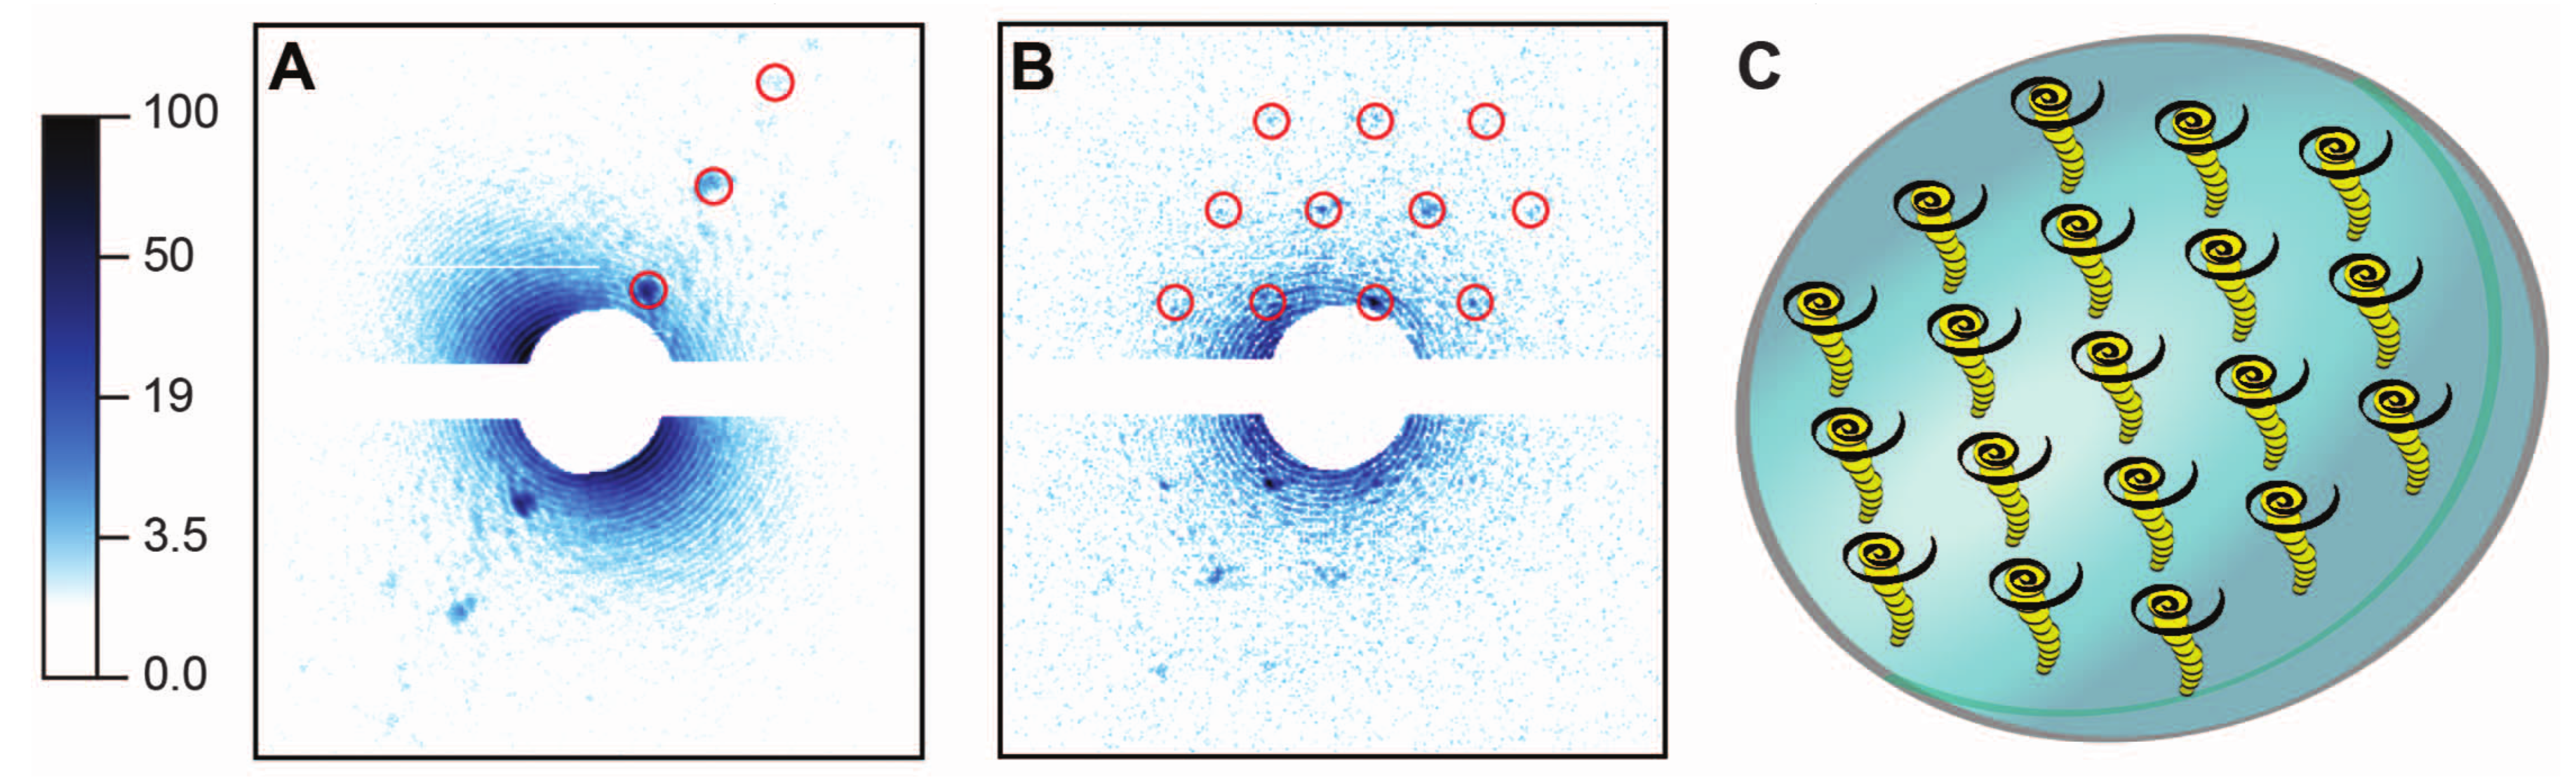
\includegraphics[width=\textwidth]{vortex-array}
				\caption{He droplets doped with Xe atoms. (A and B) X-ray diffraction images of doped droplets, displayed in a logarithmic intensity scale. (C) Droplet and embedded Xe clusters. Images in (A) and (B) correspond to tilted and parallel alignments of the vortex axes with respect to the incident x-ray beam, respectively.}
				\label{fig:vortex-array}
			\end{center}
		\end{figure}
				
		A lot of of work has been done on helium droplets the last few decades, both experimentally and theoretically. From the absorption spectra of alkali metal doped helium droplets, the study of doped mixed $^3$He--$^4$He droplets, electrons in liquid helium, to the investigation of the critical Landau velocity inside small $^4$He droplet. For a comprehensive overview of work done in the last two decades, the interested reader is referred to the review papers[JLTP.Vol142.Nos.1/2(2006), IRPC.Vol36No4.621-707(2017), IRPC.Vol33No3.301-339(2014)].

	\section{Structure of the thesis}
		\lettrine[lines=3,findent=3pt,nindent=0pt]{T}{his} thesis will consist of two parts, since the presented work focusses on two distinct areas of interest with no mutual overlap. Each part will have its own short introduction to motivate the performed research and put in a broader context. The final chapter contains a more general discussion about the presented material and will conclude with some work in progress and future prospects.

		\subsection{Part I: Excited state dynamics}
			In this part of the thesis the real-time dynamics of a single electronically excited rubidium (Rb) atom, residing in the surface dimple of a helium nano-droplet will be presented. The atom will be excited from its ground state 5s$^2\Sigma_{1/2}$ to the 5p$^2\{\Sigma,\Pi\}$ and 6p$^2\{\Sigma,\Pi\}$ manifold. This will be a combined experimental and theoretical study. The results are presented in two published articles:\\
		
			\emph{Imaging Excited-State Dynamics of Doped He Nanodroplets in Real-Time} will focus on imaging and characterising the dynamics using femtosecond spectroscopy and  time-dependent density functional theory.\\
		
			\emph{Desorption dynamics of RbHe-exciplexes off He nanodroplets induced by spin relaxation} is a combined experimental and theoretical investigation of the formation of free RbHe-exciplex molecules from laser-excited Rb-doped He nanodroplets through the mechanism of electronic spin relaxation. The role of relaxation of internal degrees of freedom of the RbHe exciplex in the desorption process has not been explicitly addressed.

		\subsection{Part II: Collisions and capture by quantised vortices}
			The second part investigates the real-time capture process of single xenon and argon atoms in their ground state by $^4$He$_{1000}$ droplets. Specifically it will address the interaction between a captured xenon or argon atom and a single quantised vortex line in the interior of the droplet. It will contain only theoretical investigations. The results will also be presented in two published works:\\
		
			\emph{Head-on Collisions of Xe Atoms Against Superfluid $^4\!$He Nanodroplets} studies the kinematics of head-on collisions between a xenon atom and a helium droplet. This scenario is then compared to a previous study of the same process with caesium to get a clear picture of the differences in dynamic behaviour between heliophilic and heliophobic species in said process. It also investigates different velocity regimes.\\
		
			\emph{Capture of Xe and Ar atoms by quantized vortices in $^4\!$He nanodroplets} addresses the capture of xenon and argon atoms at different velocity regimes and impact factors to determine the effective cross section for capture. This investigation then repeated with a dropet hosting one quantised line vortex. Also some preliminary results are presented for a larger droplet hosting an array of 6 line vortices, lined with argon atoms.

\chapter{The DFT method for heavy impurities}\label{sec:dft-method}
	\epigraph{One Functional to rule them all,
				One Functional to find them,
				One Functional to bring them all
				and in a droplet bind them
				in the Realm of Physics where Reason lies.}{\textit{some guy from LCAR}}

	\lettrine[lines=3,findent=3pt,nindent=0pt]{F}{rom} the theoretical point of view, superfluid helium must be considered as a high dimensional quantum system. Quantum Monte Carlo (QMC) \cite{Kro02} and direct quantum mechanical \cite{deL06,deL10,Agu13} calculations are the most accurate methods, but their computational demand quickly exceeds currently available computer resources when the number of helium atoms increases. Furthermore, QMC cannot describe dynamic evolution of superfluid helium in real time. To address these limitations, semi-empirical methods based on  density functional theory (DFT) formalism have been introduced \cite{Str87a,Str87b,Dal95}. DFT can be applied to much larger systems than QMC and allows for time-dependent formulation. As such, it offers a good compromise between accuracy and computational feasibility. The main drawback of DFT is that the exact energy functional is not known and must therefore be constructed in a semi-empirical manner. Moreover, doped helium droplets are limited to a mean-field description of the dopant-helium interaction. Nevertheless, DFT is the only method to date that can successfully reproduce results from a wide range of time-resolved experiments in superfluid helium on the atomic scale.\\
		
	The starting point for the density functional method are the Hohenberg-Kohn (H--K) theorems \cite{Hoh64}, which state that the total energy $E$ of a many-body quantum system at $T=0$ is a unique functional of the one-particle density
	\begin{align}
		E[\rho] = {\cal T}[\rho] +\int\!{\cal E}[\rho]\diff{r} \label{eq1}
	\end{align}
	with
	\begin{align}\label{eq:density-operator}
		\rho({\mathbf r})= \ev**{\hat\rho(\vec{r})}{\Phi} \vcentcolon= \ev**{\sum _{i=1}^{N}\delta({\mathbf r}-{\mathbf r}_i)}{\Phi}
	\end{align}
	the atomic density and $\Phi$ the many-body wave function. Here the total energy is split in a kinetic part ${\cal T}[\rho]$ and a potential part encoding the interactions. Furthermore, this unique functional gives the ground state energy if and only if the input density is the true ground state density of the system. Kohn and Sham later reformulated the theory such that we can regard the $N$-body ensemble of particles as a fictitious system of non-interacting particles, rewriting the above functional 
	\begin{equation}
		E[\rho] = T[\rho] + \int\!{\cal E}_c[\rho]\diff{r} \label{eq:ks-tot-energy}
	\end{equation}
	where this time
	\begin{equation}
		T= -\frac{\hbar^2}{2m} \sum_i \int\! \varphi_i^*({\mathbf r})\laplacian \varphi_i({\mathbf r})\diff{r} \label{eq:kin-energy}
	\end{equation}
	is the kinetic energy of this fictitious system and $\{\varphi_i\}$ are the single particle Kohn-Sham (K--S) orbitals corresponding to the non-interacting many-body wave function $\Phi(\vec{r}_1,\vec{r}_2,\ldots,\vec{r}_N)=\prod_i\varphi_i(\vec{r}_i)$. Plugging this into the definition (Eq. \ref{eq:density-operator}) of the density operator it is straightforward to show that the density of this system is $\rho(\vec{r})=\sum_i\absolutevalue{\varphi_i(\vec{r})}^2$. The difference of the true kinetic energy and the fictitious one $\mathcal{T}[\rho]-T[\rho]$ has been included in the ``correlation energy density'' term $\mathcal{E}_c[\rho]$.\\
	
	In our calculations $T=0\unit{K}$ and we therefore assume complete Bose-Einstein condensation. In this case all the helium atoms occupy the single-particle orbital $\varphi_0$ and the density becomes $\rho(\vec{r})=N\absolutevalue{\varphi_0(\vec{r})}^2$. As explained before in Section \ref{sec:bogol-order}, it is customary to define an order parameter $\Psi(\vec{r})\vcentcolon=\sqrt{\rho(\vec{r})}=\sqrt{N}\varphi_0(\vec{r})$ (see Eq. \ref{eq:order-param-real}) for a BEC, which is sometimes called the \emph{effective}- or \emph{macroscopic wave function}. The expression for the kinetic energy (Eq. \ref{eq:kin-energy}) then simplifies to
	\begin{align}
		T[\rho] =
		-\frac{\hbar^2}{2m} N \ev**{\laplacian}{\varphi_0} = \frac{\hbar^2}{2m} \int\! \abs{\grad{\Psi}}^2\diff{r} \label{eq5}
	\end{align}
	
	To describe the time evolution of the system, the Runge-Gross theorem extends DFT in its time-dependent version TDDFT [40]. The minimisation of the total energy (Eq. \ref{eq:ks-tot-energy}) leads to the following time-dependent Euler-Lagrange (EL) equation 
	\begin{align}
		i\hbar\frac{\partial}{\partial t} \Psi({\mathbf r},t) = \left\{-\frac{\hbar^2}{2m}\laplacian + \fdv{\mathcal{E}_c}{\rho}\right\}\Psi(\textbf{r},t) \vcentcolon= {\cal H}\left[\rho\right]\Psi(\textbf{r},t) 
		\label{eq:td-el-equation}
	\end{align}
	As long as we are in the thermodynamic regime the solutions $\Psi(\textbf{r},t)$ can be decomposed into the liquid's density an associated velocity potential field (see Section \ref{sec:bogol-order}, \ref{sec:rot-vort}).\\
	
	Considering only eigenstates $\Psi(\vec{r},t)=\Psi_0(\vec{r})\unit{e}^{-i\mu t/\hbar}$ of the time-independent Hamiltonian ${\cal H}\left[\rho\right]$ the time-dependent EL-equation reduces to a time independent one
	\begin{align}
		\left\{-\frac{\hbar^2}{2m} \laplacian + \fdv{\mathcal{E}_c}{\rho}\right\}\Psi_0(\textbf{r}) = \mu\Psi_0(\textbf{r})
		\label{eq:el-equation}
	\end{align}
	with $\mu$ the chemical potential. Solving this equation by iteration will result in the ground state density $\abs{\Psi_0}^2$ of the system. Within the H--K framework and the variation principle that was used to obtain these EL-equations, the nature of the minimisation is such that it gives the lowest energy for a given symmetry. This means that as long as the input state doesn't break the symmetry of the time-independent EL-equation, it minimises the energy of this state even if it doesn't lead to the ground state. This can be used to obtain a stationary vortex-line solution. With the inclusion of appropriate constraints in the energy functional the same procedure can be used to obtain helium densities with an array of vortex-lines.   

	\section{The Orsay--Trento Density Functional}
		\begin{table}[t]
			Model parameters for the OT-DFT and solid functionals.
			\vspace{50pt}
			{\begin{tabular}{@{}lccccc}
				\hline
				\hline
				$\epsilon_{LJ}$  (K)    & $\sigma$ (\AA)& $h$ (\AA) & $c_2$ (K \AA$^6$)  & $c_3$ (K \AA$^9$) & $\alpha_s$ (\AA$^3$) \\
				 10.22   & 2.556 & 2.190323 & $-$2.41186 $\times 10^4$ & 1.85850 $\times 10^6$ & 54.31 \\
				\hline
				 $\rho_{0s}$ (\AA$^{-3}$)& $l$ (\AA)&$C$ (Hartree) &$\beta$ (\AA$^3$) & $\rho_m$ (\AA$^{-3}$) & $\gamma_{11}$ \\  
				  0.04& 1. & 0.1 &40.   & 0.37 & $-$19.7544 \\
				  \hline
				  $\gamma_{12}$ (\AA$^{-2}$)& $\alpha_1$  (\AA$^{-2}$) & $\gamma_{21}$  & $\gamma_{22}$ (\AA$^{-2}$) & $\alpha_2$ (\AA$^{-2}$) &      \\  
				   12.5616 &1.023 &  $-$0.2395 & 0.0312 & 0.14912  & \\
				\hline
				\hline
			\end{tabular}}
			\label{table1}
		\end{table}

		\begin{figure}[t]
			\begin{center}
				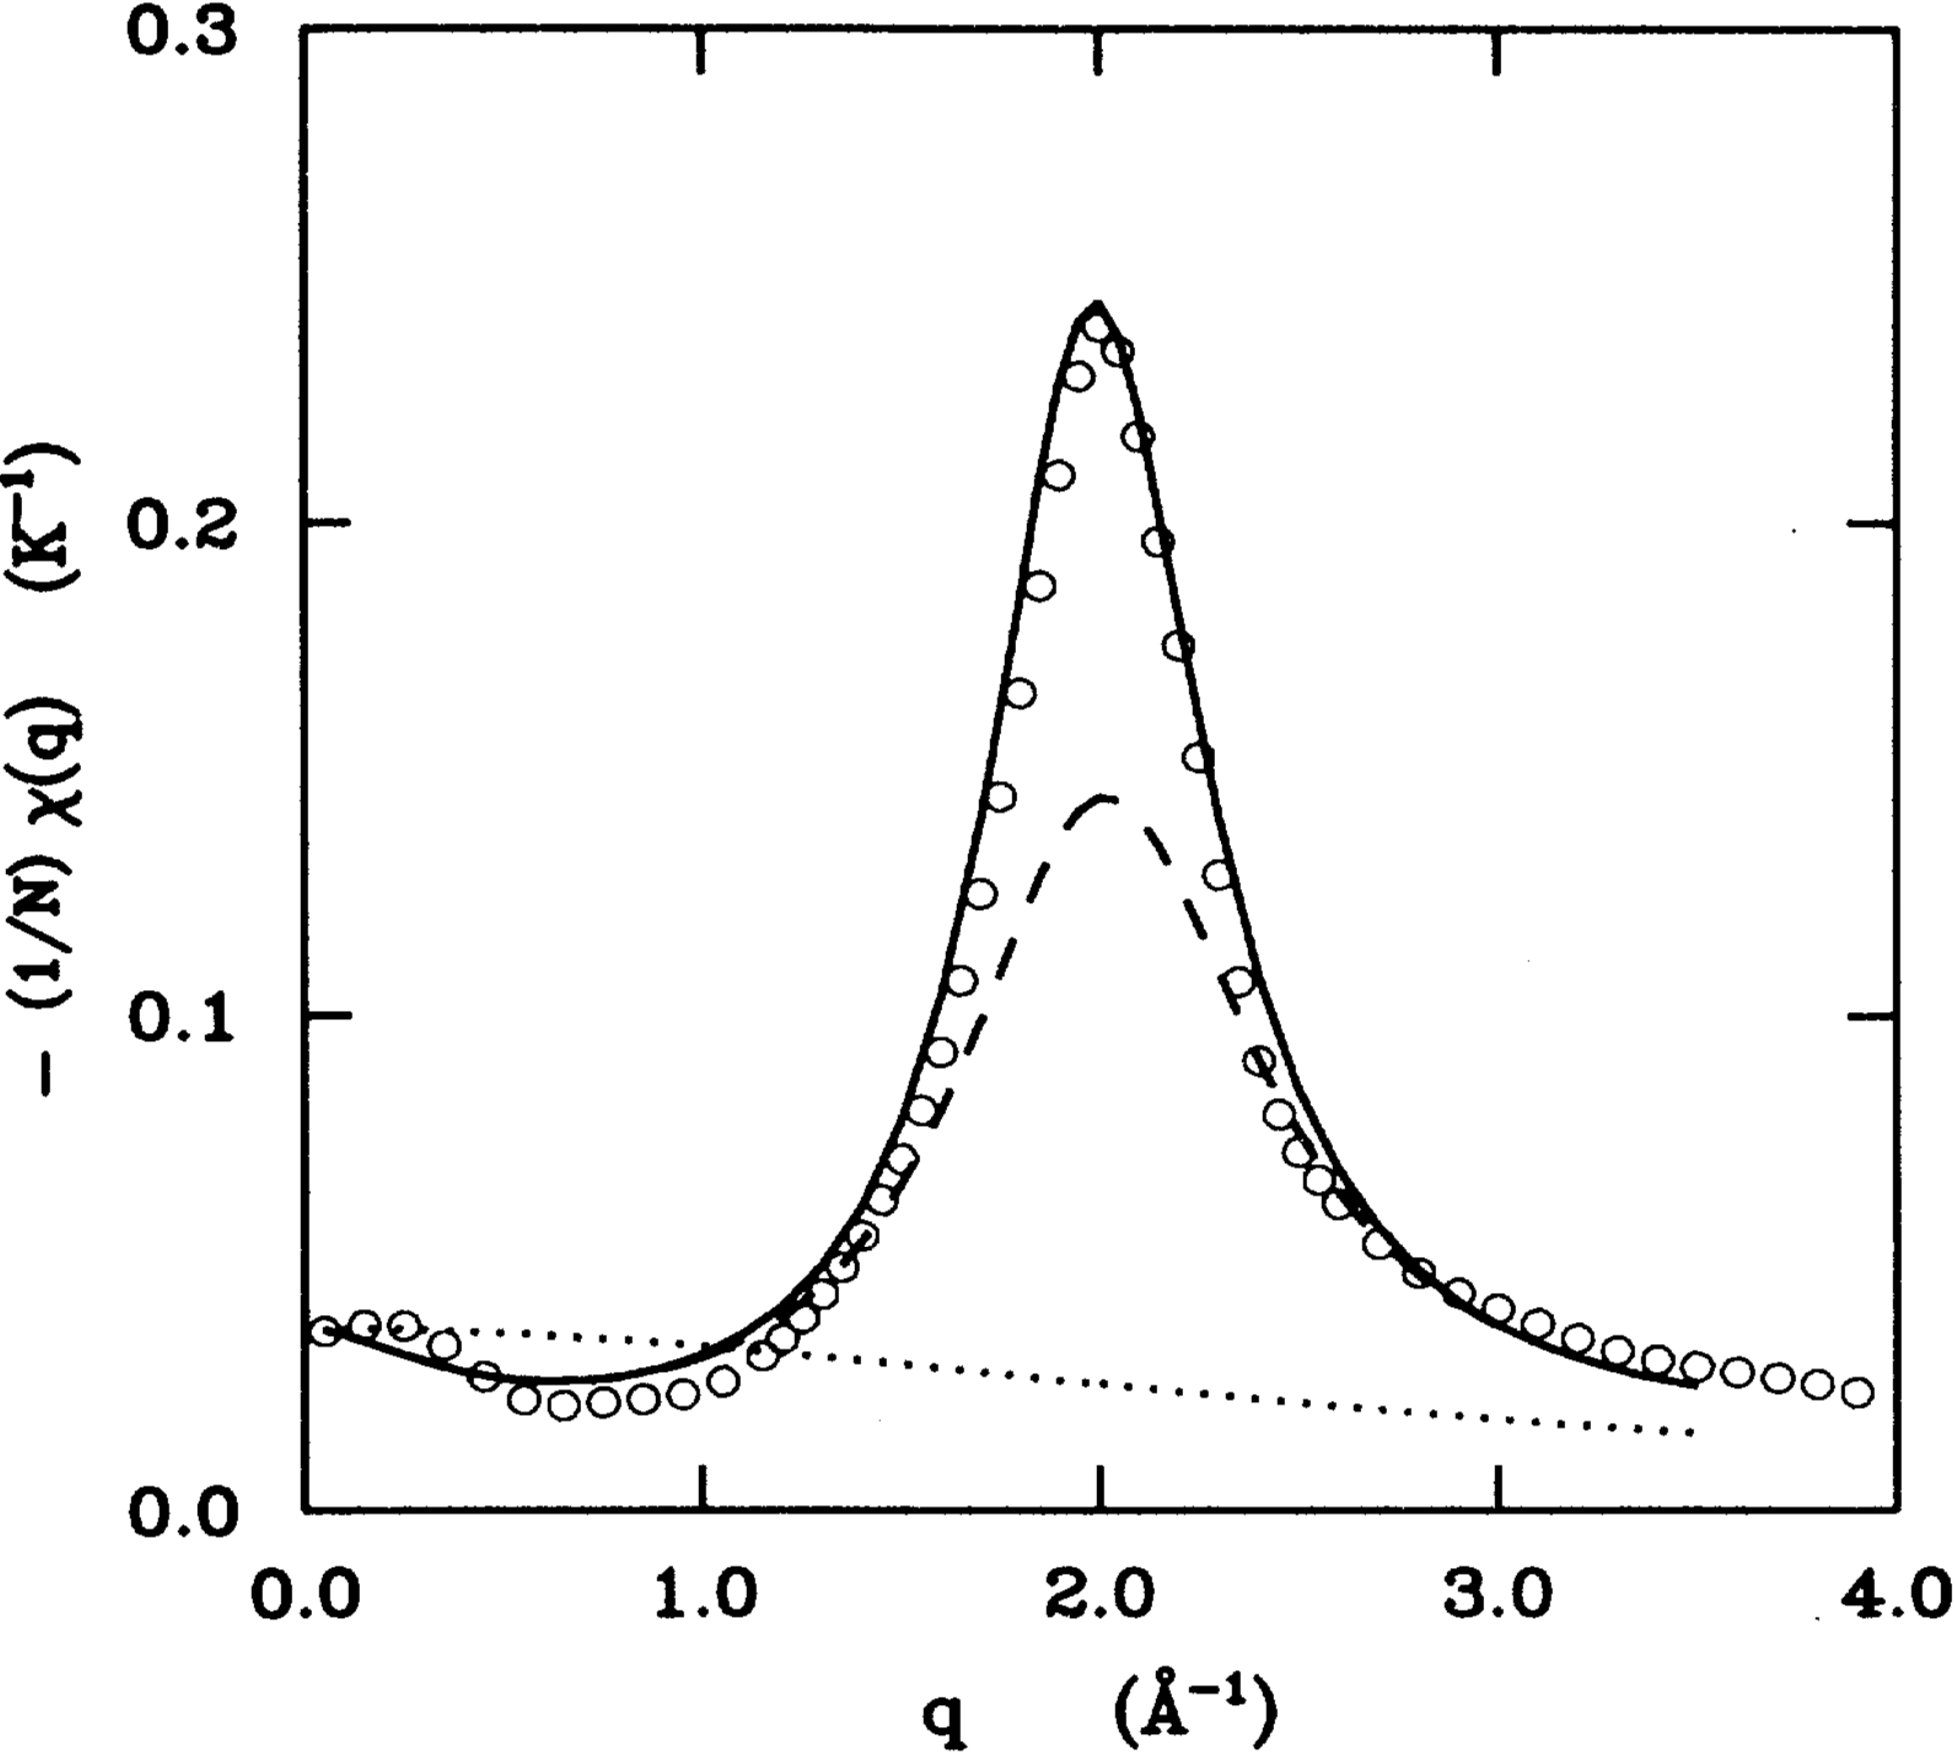
\includegraphics[width=0.75\textwidth]{static-response-function}
				\caption{Static response function of liquid $^4$He at zero pressure. Points: experimental data; dotted line: from functional of refs 15,16; dashed line: OP functional ref 1; solid line present functional.}
				\label{fig:static-response-function}
			\end{center}
		\end{figure}
			
		\lettrine[lines=3,findent=3pt,nindent=0pt]{T}{he} functional that is used in the work presented in this thesis is based on the Orsay-Trento (OT) functional. It uses a finite-range, non-local approach and it is, to date the most accurate model in the sense that it accurately reproduces bulk properties of liquid helium at $T=0=P$, written as		
		\begin{align}
			{\cal E}_c[\rho ,\mathbf{v}] &=  
			\frac{1}{2} \left.\int \! \right\{\rho({\bf r}) V_{LJ}(|{\bf r}-{\bf r'}|) \rho({\bf r'}) \nonumber \\
			&+ \left.\frac{1}{2} c_2\, \rho({\bf r}) \left[{\bar \rho}({\bf r}) \right]^2 
			+ \frac{1}{3} c_3 \, \rho({\bf r}) \left[ {\bar \rho}({\bf r}) \right]^3\right\}\diff{r'} \nonumber \\
			&- \frac{\hbar^2}{4m} \alpha_s \int \! F(|{\bf r}-{\bf r'}|) \left[ 1- \frac{{\tilde \rho}({\bf r})}{\rho_{0s}} \right]\grad{\rho({\bf r})} \cdot \grad{\rho({\bf r'})} \left[ 1- \frac{{\tilde \rho}({\bf r'})}{\rho_{0s}} \right]\diff{r'} \nonumber \\
			& - \frac{m}{4} \int \! V_J(| \mathbf{r} - \mathbf{r}'|)\, \rho(\mathbf{r}) \, \rho(\mathbf{r}')\,  [\mathbf{v}(\mathbf{r})-\mathbf{v}(\mathbf{r}')]^2\diff{r'} \label{eq:otf}
		\end{align}
		The first term corresponds to a classical Lennard-Jones type two-body interaction between the helium atoms. The interaction is screened at short distances where the interaction energy is of the same order as the correlation effects:
		\begin{align}
			V_{LJ}(r) = \begin{cases}
			\epsilon_{LJ} \left[\left(\frac{\sigma}{r} \right)^{12} - \left(\frac{\sigma}{r} \right)^{6} \right] & {\rm if} \quad r > h \\
			0 & {\rm otherwise}
			\end{cases}\label{eq9}
		\end{align}
		In the second line, the terms corresponding to $c_2$ and $c_3$, correct for short range correlations when $r<h$. The weighted density $\bar{\rho}$ is the average density $\rho$ over a sphere of radius $h$:
		\begin{align}
			\bar{\rho}(\vec{r}) = \int\!\Pi_h\qty(\abs{\vec{r}-\vec{r'}})\rho({\vec{r'}})\diff{r'},
		\end{align}
		with
		\begin{align}
			\Pi_h(r) \vcentcolon= \begin{cases}
				\frac{3}{4\pi h^3} & \rm{if} \quad r\leq h \\
				0 & \rm{otherwise}
			\end{cases}
		\end{align}
		The third line is a non-local correction to the kinetic energy (KC). It partially accounts for the difference $\mathcal{T}[\rho]-T[\rho]$ mentioned in the previous section. The gradient-gradient interaction function $F$ is a Gaussian kernel defined as
		\begin{align}
			F(r) = \frac{1}{l^3\sqrt{\pi^3}}\unit{e}^{-r^2/l^2}
		\end{align}
		All the parameters are fixed to reproduce the peak of the static response function (see Fig.  ) in the bulk liquid. The factor $\qty(1-\tilde{\rho}/\rho_{0s})$ is included to match the pressure dependence of the static response function predicted by diffusion Monte Carlo calculations [ref 21 in OT paper]. The quantity $\tilde{\rho}(\vec{r})$ is another weighted density, calculated using $F$ as a weight
		\begin{align}
			\tilde{\rho}(\vec{r}) \vcentcolon= \int\!F\qty(\abs{\vec{r}-\vec{r'}})\rho(\vec{r'})\diff{r'}
		\end{align}
		The density $\tilde{\rho}(\vec{r})$ is very close to the normal density $\rho(\vec{r})$ except in very inhomogeneous situations. For helium droplets one can safely use $\rho$ instead of $\tilde{\rho}$.\\
			
		Finally, in the last line in Eq. \ref{eq:otf} is called the \emph{back-flow} term and influences the dynamic response of the system. It plays the role of a non-local kinetic energy. Since the back-flow contains the factor $\vec{v}-\vec{v'}$, as defined in Eq. \ref{eq:velocity-field} the contribution will only be non-zero whenever the order parameter $\Psi$ is complex-valued. Which means that in the time-independent case this will only affect the vortex states. The phenomenological effective current-current interaction $V_J(r)$ is calibrated so that it reproduces the experimental phonon-roton spectrum (see Fig. \ref{fig:dispersion-relation}):
		\begin{align}
			V_J(r) =\,&(\gamma_{11} +\gamma_{12} \, r^2) e^{-\alpha_1 r^2}\\
				+\,&(\gamma_{21} +\gamma_{22} \, r^2) e^{-\alpha_2 r^2}
			\label{eq15}
		\end{align}
		All the parameters of the functional are given in Table \ref{table1}.

		\subsection{The Solid-OT Density Functional}
			In the presence of highly inhomogeneous liquid densities, e.q. atomic impurities with a very strong He-X interaction, the OT-functional Eq. (\ref{eq:otf}) becomes numuerically unstable. To deal with this problem an additional cut-off can be used
			\begin{align}
				\mathcal{E}_\mathrm{sol} \vcentcolon= C\rho(\vec{r})\qty{1+\tanh(\beta\qty[\rho(\vec{r})-\rho_\mathrm{m}])}
			\end{align}
			where the model parameters $\qty{C,\beta,\rho_\mathrm{m}}$ are specified in Table \ref{table1}. Including this term in the OT-functional prevents excessive density build-up. $\mathcal{E}_\mathrm{sol}$ only starts to deviate from zero whenever the liquid density $\rho$ is comparable to $\rho_\mathrm{m}$ or larger. Therefore, inclusion of this term in the functional does not alter the density distribution. This penalty term was originally developed to account for the liquid-solid phase transition of $^4$He[61,62]. The functional that has been used to obtain the result presented in thus work is what we call the ``Solid-OT-DFT functional''. It consists of the first three terms of the original OT-functional Eq. (\ref{eq:otf}), plus $\mathcal{E}_\mathrm{sol}$
			\begin{align}
				{\cal E}_c^{sol}[\rho] &=  
				\frac{1}{2} \left.\int \! \right\{\rho({\bf r}) V_{LJ}(|{\bf r}-{\bf r'}|) \rho({\bf r'}) \nonumber \\
				&+ \left.\frac{1}{2} c_2\, \rho({\bf r}) \left[{\bar \rho}({\bf r}) \right]^2 
				+ \frac{1}{3} c_3 \, \rho({\bf r}) \left[ {\bar \rho}({\bf r}) \right]^3\right\}\diff{r'} \nonumber \\
				&+ C\rho(\vec{r})\qty\Big{1+\tanh(\beta\qty[\rho(\vec{r})-\rho_\mathrm{m}])} \label{eq:solid-otf}
			\end{align}

	\section{Static calculations}
		\lettrine[lines=3,findent=3pt,nindent=0pt]{I}{n} the work presented here all the impurities are heavy compared to the mass of $^4$He, e.g. the mass of Rubidium is about 21 times larger than that of Helium, Xenon roughly 33 times and Argon about 10 times. Therefore we will treat the centre of mass motion of the impurities as classical. In the DFT derived EL-equations this will be modelled as an external field $V_X$
		\begin{align}
			E[\rho] \rightarrow E[\rho] +  \int\!\rho({\mathbf r}) V_X\qty(\abs{{\mathbf r} - {\mathbf r}_I})\diff{r} \label{eq:el-static-hi}
		\end{align}
		where $X$ is the label of the used $^4$He--impurity pair interaction and ${\vec r}_I$ is the position of the impurity. Varying the modified functional to minimise the energy one now finds a new EL-equation in which the helium--impurity interaction is included:
		\begin{align}
			\left\{-\frac{\hbar^2}{2m_4} \laplacian + \fdv{\mathcal{E}_c}{\rho} + V_X(|{\mathbf r} - {\mathbf r_I}|)\right\}\Psi({\mathbf r}) = \mu \Psi({\mathbf r}) \label{eq:el-static-hi}
		\end{align}
		This equation is then solved in a self-consistent way by the Imaginary Time Method[ref 69] (ITM) in cartesian coordinates upon convergence. The calculations are performed in three dimensions without imposing any symmetries that are present in the external potential. All the quantities are discretised on evenly spaced cartesian grid with a grid constant that is typically of the order of $0.4\unit{\AA}$. The differential operators are evaluated using a $k$-point finite difference method where most of the time $k=13$ is sufficiently accurate. The integrals in the density-functional can be expressed as convolutions and can therefore be evaluated in momentum-space by exploiting the convolution theorem, using proprietary highly optimised parallel Fast Fourier Transform algorithms. 
			
		\subsection{Producing vortical states}\label{sec:vortical-states}
			The helium density that minimises the energy of the vortical states $\Psi_s$ (Eq. \ref{eq:line-vortex}), introduced in Section \ref{sec:rot-vort} can be obtained by solving the same EL-equation as for a vortex-free droplet. This becomes more clear when we write Eq. (\ref{eq:el-equation}) in cylindrical coordinates and then substitute $\Psi_0$ by $\Psi_s$:
			\begin{align}
				\qty{-\frac{\hbar^2}{2m}\qty[\frac{1}{r}\pdv{r}\qty(r\pdv{r})-\frac{s^2}{r^2}]+\fdv{\mathcal{E}_c}{\rho}}\Psi_s(\vec{r}) = \mu\Psi_s(\vec{r}) \label{eq:el-cyl}
			\end{align}
			Written like this it is evident that the ground state $\Psi_0$ is just the special case for $s=0$. Obtaining the solution using the ITM works as long as the solution has overlap with initial guess for the order parameter. Starting with a trial order parameter similar to $\Psi_s$ will guarantee this. To do this we use the ``imprinting'' technique where we use the ground state density of a previously obtained vortex-free droplet and multiply it with a normalised complex factor
			\begin{align}
				\Psi(\mathbf{r}) = \sqrt{\rho_0(\vec{r})} \,\times \frac{x + iy}{\sqrt{x^2 + y^2}} \label{eq28}
			\end{align}
			where $\rho_0$ is the ground state density of the vortex-droplet.  In cylindrical coordinates this factor is equivalent to the one in Eq. (\ref{eq:line-vortex}) for $s=1$.\\ 
			
			This changes for droplets with two or more vortices, where the cylindrical symmetry is broken and the solutions are no longer solutions of Eq. (\ref{eq:el-cyl}) nor eigenfunctions of the angular momentum operator. In this case the time-independent EL-equation has to be modified to include a rotational constraint
			\begin{align}
				{\cal H} \rightarrow {\cal H}-\Omega \hat{L}_z
			\end{align}
			 such that for a suitable choice of $\Omega$ the vortex-array solution becomes favourable to the ground state. Since these states are no longer eigenstates of the original time-dependent Hamiltonian, these states are no longer stationary and will start to rotate with frequency $\Omega$. The initial guess for a droplet with $n_v$ vortices can be produced using the same imprinting method as mentioned before		
			\begin{align}
				\Psi(\mathbf{r})=\sqrt{\rho_0(\vec{r})} \times \prod _{j=1}^{n_v}\left[ {(x-x_j)+i(y-y_j) \over \sqrt{(x-x_j)^2+(y-y_j)^2}}  \right] \label{eq32}
			\end{align}
			where $\rho_0$ is again the ground state density of the vortex-free droplet and $(x_j,y_j)$ is the initial position of the $j$-th vortex-line parallel to the $z$-axis.

	\section{Dynamic calculations}
		\lettrine[lines=3,findent=3pt,nindent=0pt]{F}{or} the dynamic evolution of atomic impurities excited from $ns$-states to $n's$-states, we do not need to keep track of the evolution of the electronic state of the impurity since it keeps its spherically symmetric orbital. In this case we only need to describe the time evolution of the centre of mass coordinate of the impurity. As in the statics, because of the large atomic mass of the impurity compared to helium, the time evolution of the centre of mass coordinate of the impurity is treated classically. To obtain the correct energy for the whole droplet-impurity system the energy functional needs to be extended to include the impurities centre of mass motion and the impurity-helium interaction
		\begin{align}
			E[\rho] \rightarrow E[\rho] + \frac{p^2_I}{2 m_I} + \int \! \rho(\mathbf{r}) \, V_{X^{\!*}}\qty(\abs{\vec{r}-\vec{r}_I})\diff{r} \label{eq33}
		\end{align}
		where $p^2_I$ is the classical momentum of the impurity, $m_I$ is the impurity mass and $V_{X^{\!*}}$ is the X-$^4$He pair potential for a ground-, excited- or ionised state. The equations of motion for the time evolution of the order parameter $\Psi\qty(\vec{r},t)$ and the centre of mass of the impurity $\ddot{\vec{r}}_I$ are  
		\begin{align}
			i\hbar\frac{\partial}{\partial t} \Psi &= \qty[-\frac{\hbar^2}{2m_4} \laplacian +\frac{\delta {\cal E}_c}{\delta \rho} + V_{X^*}(|\mathbf{r}- \mathbf{r}_I|)]\Psi\nonumber\\
			m_I \ddot{\mathbf{r}}_I &= - \grad_{\vec{r}_I} \left[  \int \!\rho(\mathbf{r}) V_{X^*}(|\mathbf{r}- \mathbf{r}_I|)\diff{r}  \right] \nonumber \\
			&= -\int \! V_{X^*}(|\mathbf{r}- \mathbf{r}_I|)  \, \grad \rho(\mathbf{r})\diff{r} \label{eq34}
		\end{align}
	
		\subsection{The DIM model}
			\begin{figure}[t]
				\begin{center}
					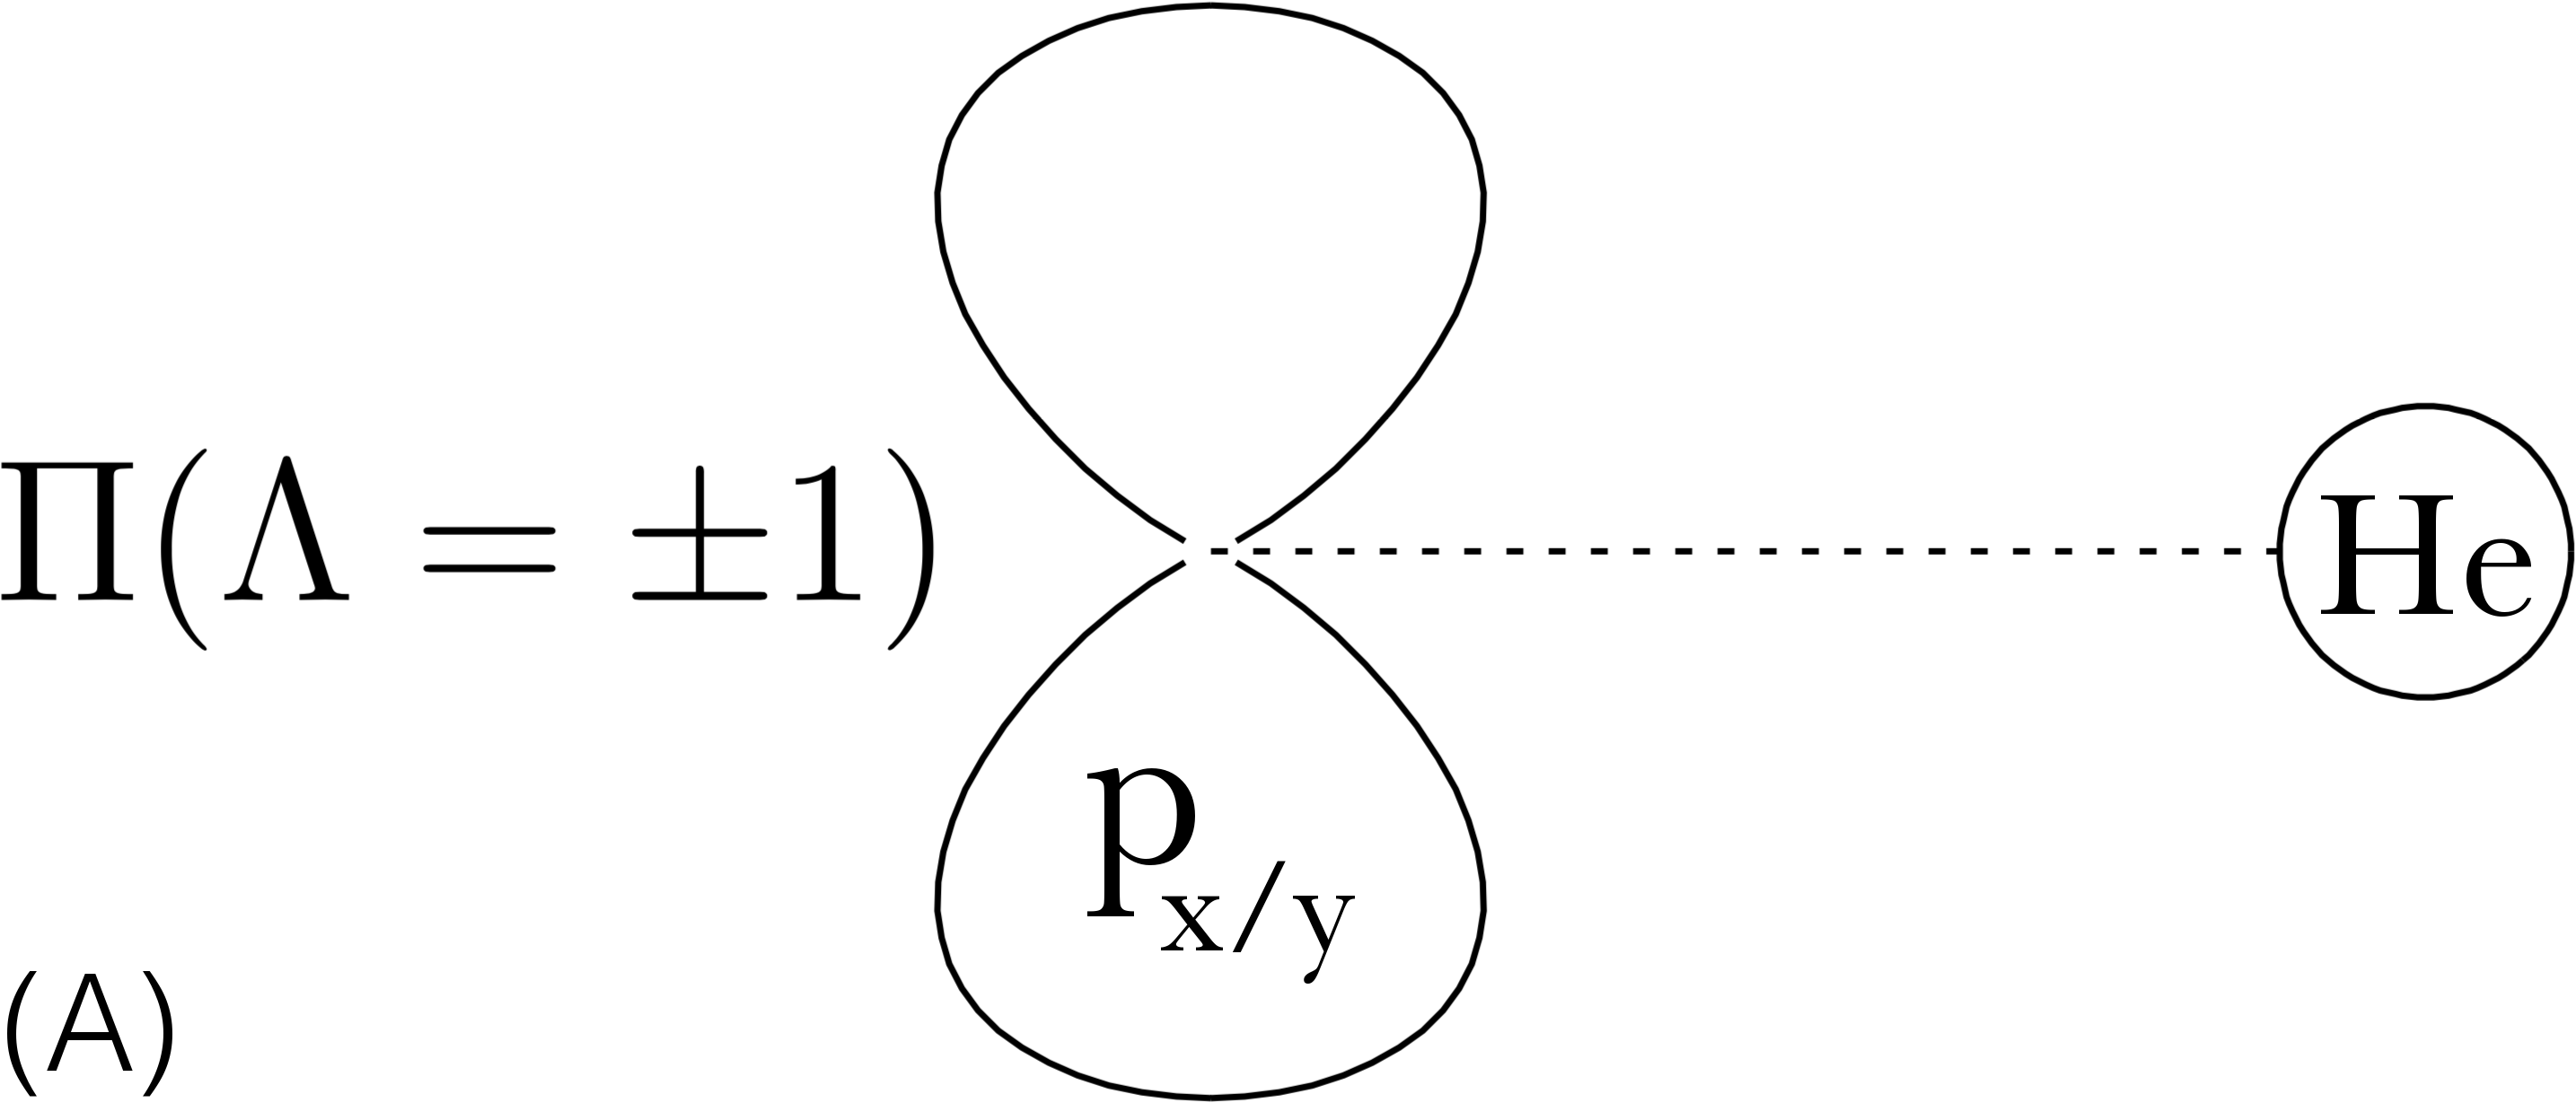
\includegraphics[width=0.45\textwidth]{pxy-he}
					\hspace{20px}
					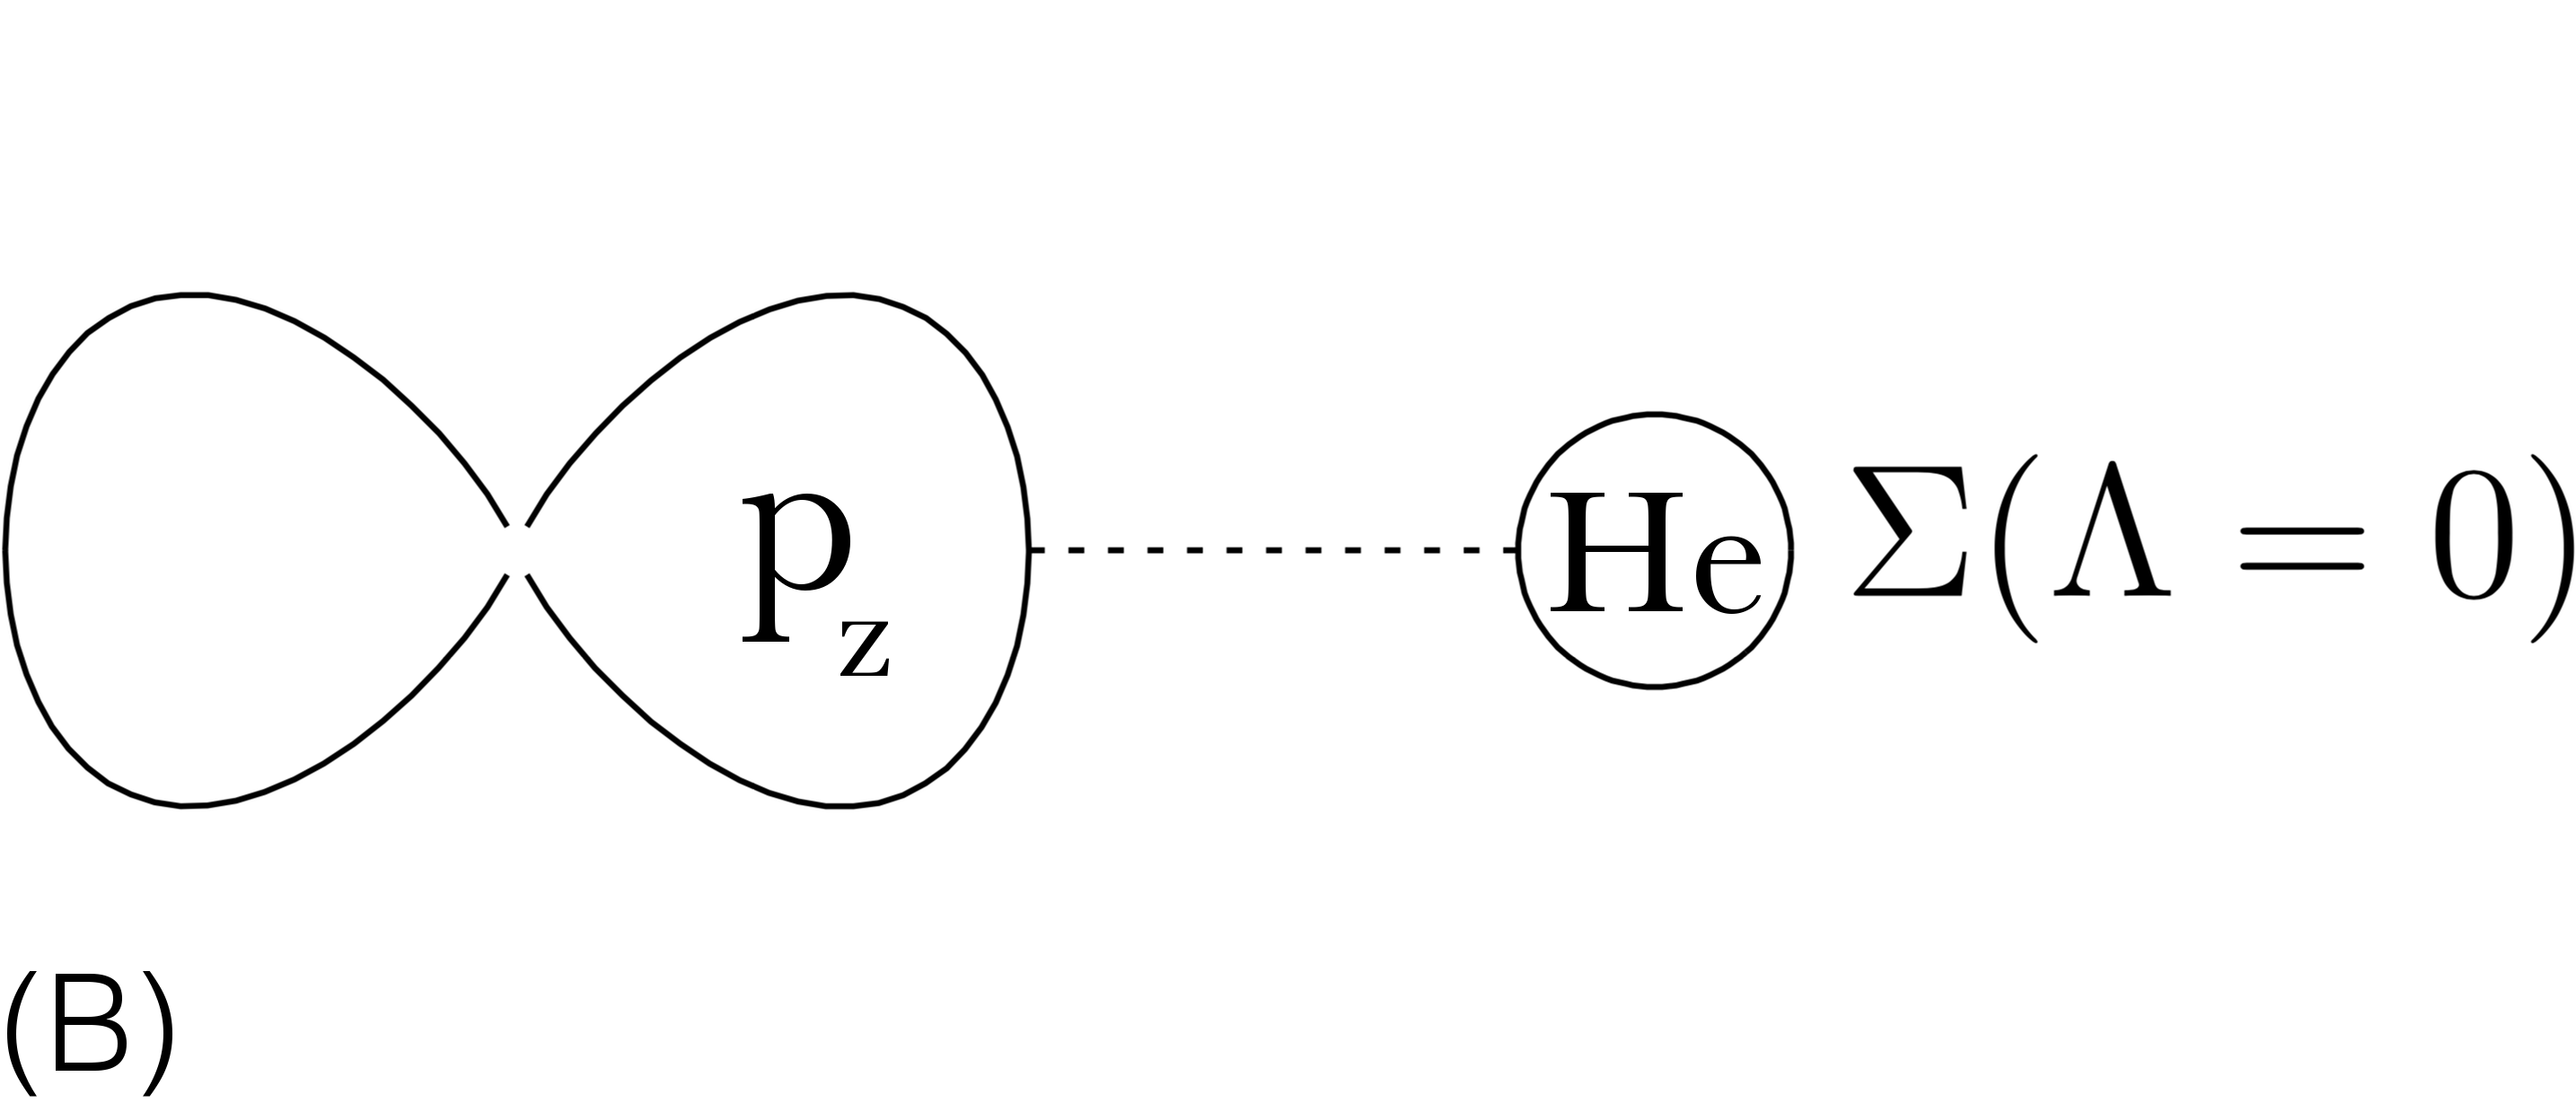
\includegraphics[width=0.45\textwidth]{pz-he}
				\end{center}
				\caption{Level splitting of the p-orbitals in the presence of helium, that breaks the spherical symmetry. (A) A double degenerate n'p$_\mathrm{x/y}$-orbital and (B) a single n'p$_\mathrm{z}$-orbital. (Illustration courtesy of M. Martinez)}
				\label{fig:p-orbitals}
			\end{figure}				
			The situation becomes slightly more complicated for $n$s-states excited to $n'$p-states (effective one-electron excited $^2$P-states). Since the p-orbital is no longer spherically symmetric, we also need to include a description for the time evolution of the orientation of the p-orbital. To do this we use the diatomic model (DIM). The interaction between a helium atom ($^1$S$_0$-state) and the triple degenerate $L=1$ electronic state of the impurity partially lifts the degeneracy so that the interaction can be decomposed into a $\Sigma$-state and a double degenerate $\Pi$-state (see Fig. \ref{fig:p-orbitals}). In the cylindrical symmetry of the DIM it is customary to use the molecular term symbol $^{2S+1}\Lambda_\Omega$ to label the levels. Here $S$ is the total spin angular momentum (and $2S+1$ the spin multiplicity), $\Lambda$ is the modulus of the total orbital angular momentum and $\Omega$ is the total angular momentum, all projected along the internuclear axis. Following the spectroscopic notation the orbitals corresponding to $\Lambda=0,1,2,3,\ldots$ are labeled $\Sigma,\Pi,\Delta,\Phi,\ldots$. The interaction between a helium atom and the impurity's electronic structure can be expressed in an uncoupled basis
			\begin{align}
				 \ket{p_{im}}\in\qty\big{\,\ket{p_{xm}}\!,\ket{p_{ym}}\!,\ket{p_{zm}}} \label{eq:dim-basis}
			\end{align}
			of real one-electron p-orbitals oriented along the internuclear axis (see Fig. \ref{fig:dim-axes}). The helium-impurity interaction matrix is given by
			\begin{align}
				\mathcal{V}^{DIM}(r_m) &= V_{\Pi}(r_m)\qty\big(\dyad{p_{xm}}+\dyad{p_{ym}})+V_{\Sigma}(r_m)\dyad{p_{zm}} \nonumber \\
					&= V_{\Pi}(r_m)\qty\big(\mathbb{1}_3-\dyad{p_{zm}})+V_{\Sigma}(r_m)\dyad{p_{zm}} \nonumber \\
					&=V_{\Pi}(r_m)\mathbb{1}_3+\qty\big[V_{\Sigma}(r_m)-V_{\Pi}(r_m)]\dyad{p_{zm}}
			\end{align}	
			where $r_m$ is the modulus of the interatomic separation vector and $V_\Pi$ and $V_\Sigma$ are the $\Pi$ and $\Sigma$ impurity-He pair potentials in the absence of spin-orbit coupling. For a system consisting of $N$ helium atoms the total interaction energy is calculated by summing over all the contributions of the $N$ individual $^4$He--X contributions (DIM \cite{82})
			\begin{align}
				\mathcal{U}^{DIM}(\vec{r}_I)=\sum_{m=1}^{N}\mathcal{V}^{DIM}(r_m)
			\end{align}
			It is more convenient to express the interaction in a basis common to all impurity-helium pairs, instead of a basis that depends on the particular impurity-helium pair chosen. To do this we apply a rotation $\mathcal{R}_m:\hat{\vec{z}}_m\mapsto\hat{\vec{z}}\propto\vec{r}_I$, so that the matrix corresponding to the $m^{\rm th}$ $^4$He atom expressed in the common basis is given by
			\begin{align}
				\dyad{p_{zm}} = \mathcal{R}_m\dyad{p_z}\mathcal{R}_m^{-1}
			\end{align}
			It can be shown that the elements of this matrix in cartesian coordinates are of the form
			\begin{equation}
				\mel**{p_i}{\mathcal{R}_m\dyad{p_z}\mathcal{R}_m^{-1}}{p_j} = \frac{r_{im}\,r_{jm}}{\norm{\vec{r}_m}^2}		\label{eq39}
			\end{equation}	
			where $(i,j)\in\qty{x,y,z}$. With these definitions we can write the matrix elements $U^{DIM}_{ij}$ of the interaction energy $\mathcal{U}^{DIM}$
			\begin{align}
				U^{DIM}_{ij}(\vec{r}_I)=\mel**{p_i}{\mathcal{U}^{DIM}}{p_j} = \sum_{m=1}^{N} V^{DIM}_{ij}(r_m)
			\end{align}
			where
			\begin{align}
				V^{DIM}_{ij}(r_m) \vcentcolon= \qty{V_\Pi(r_m)\delta_{ij}+\qty\big[V_\Sigma(r_m)-V_\Pi(r_m)]\frac{r_{im}\,r_{jm}}{\norm{\vec{r}_m}^2}} \label{eq:vdim}
			\end{align}
			are the matrix elements of $\mathcal{V}^{DIM}$ expressed in the common basis. Since we are working with a continues helium density $\rho(\vec{r})$ and not with discrete atoms the summation over $N$ helium atoms in the previous expression is replaced by an integral over the density $\sum_m\rightarrow\int\!\rho(\vec{r})\diff{r}$ which finally gives for the matrix element $U^{DIM}_{ij}$
			\begin{align}
				U^{DIM}_{ij}(\vec{r}_I) = \int\! \rho\qty(\vec{r}+\vec{r}_I)\,V^{DIM}_{ij}(r)\diff{r}
			\end{align}
			
			The eigenvalues $U^{\mathrm{np}}_k(\vec{r}_I)$ of this real symmetric matrix define the potential energy curves (PECs) as a function of the distance between the surrounding helium and the impurity.
			\begin{figure}[t]
				\begin{center}
					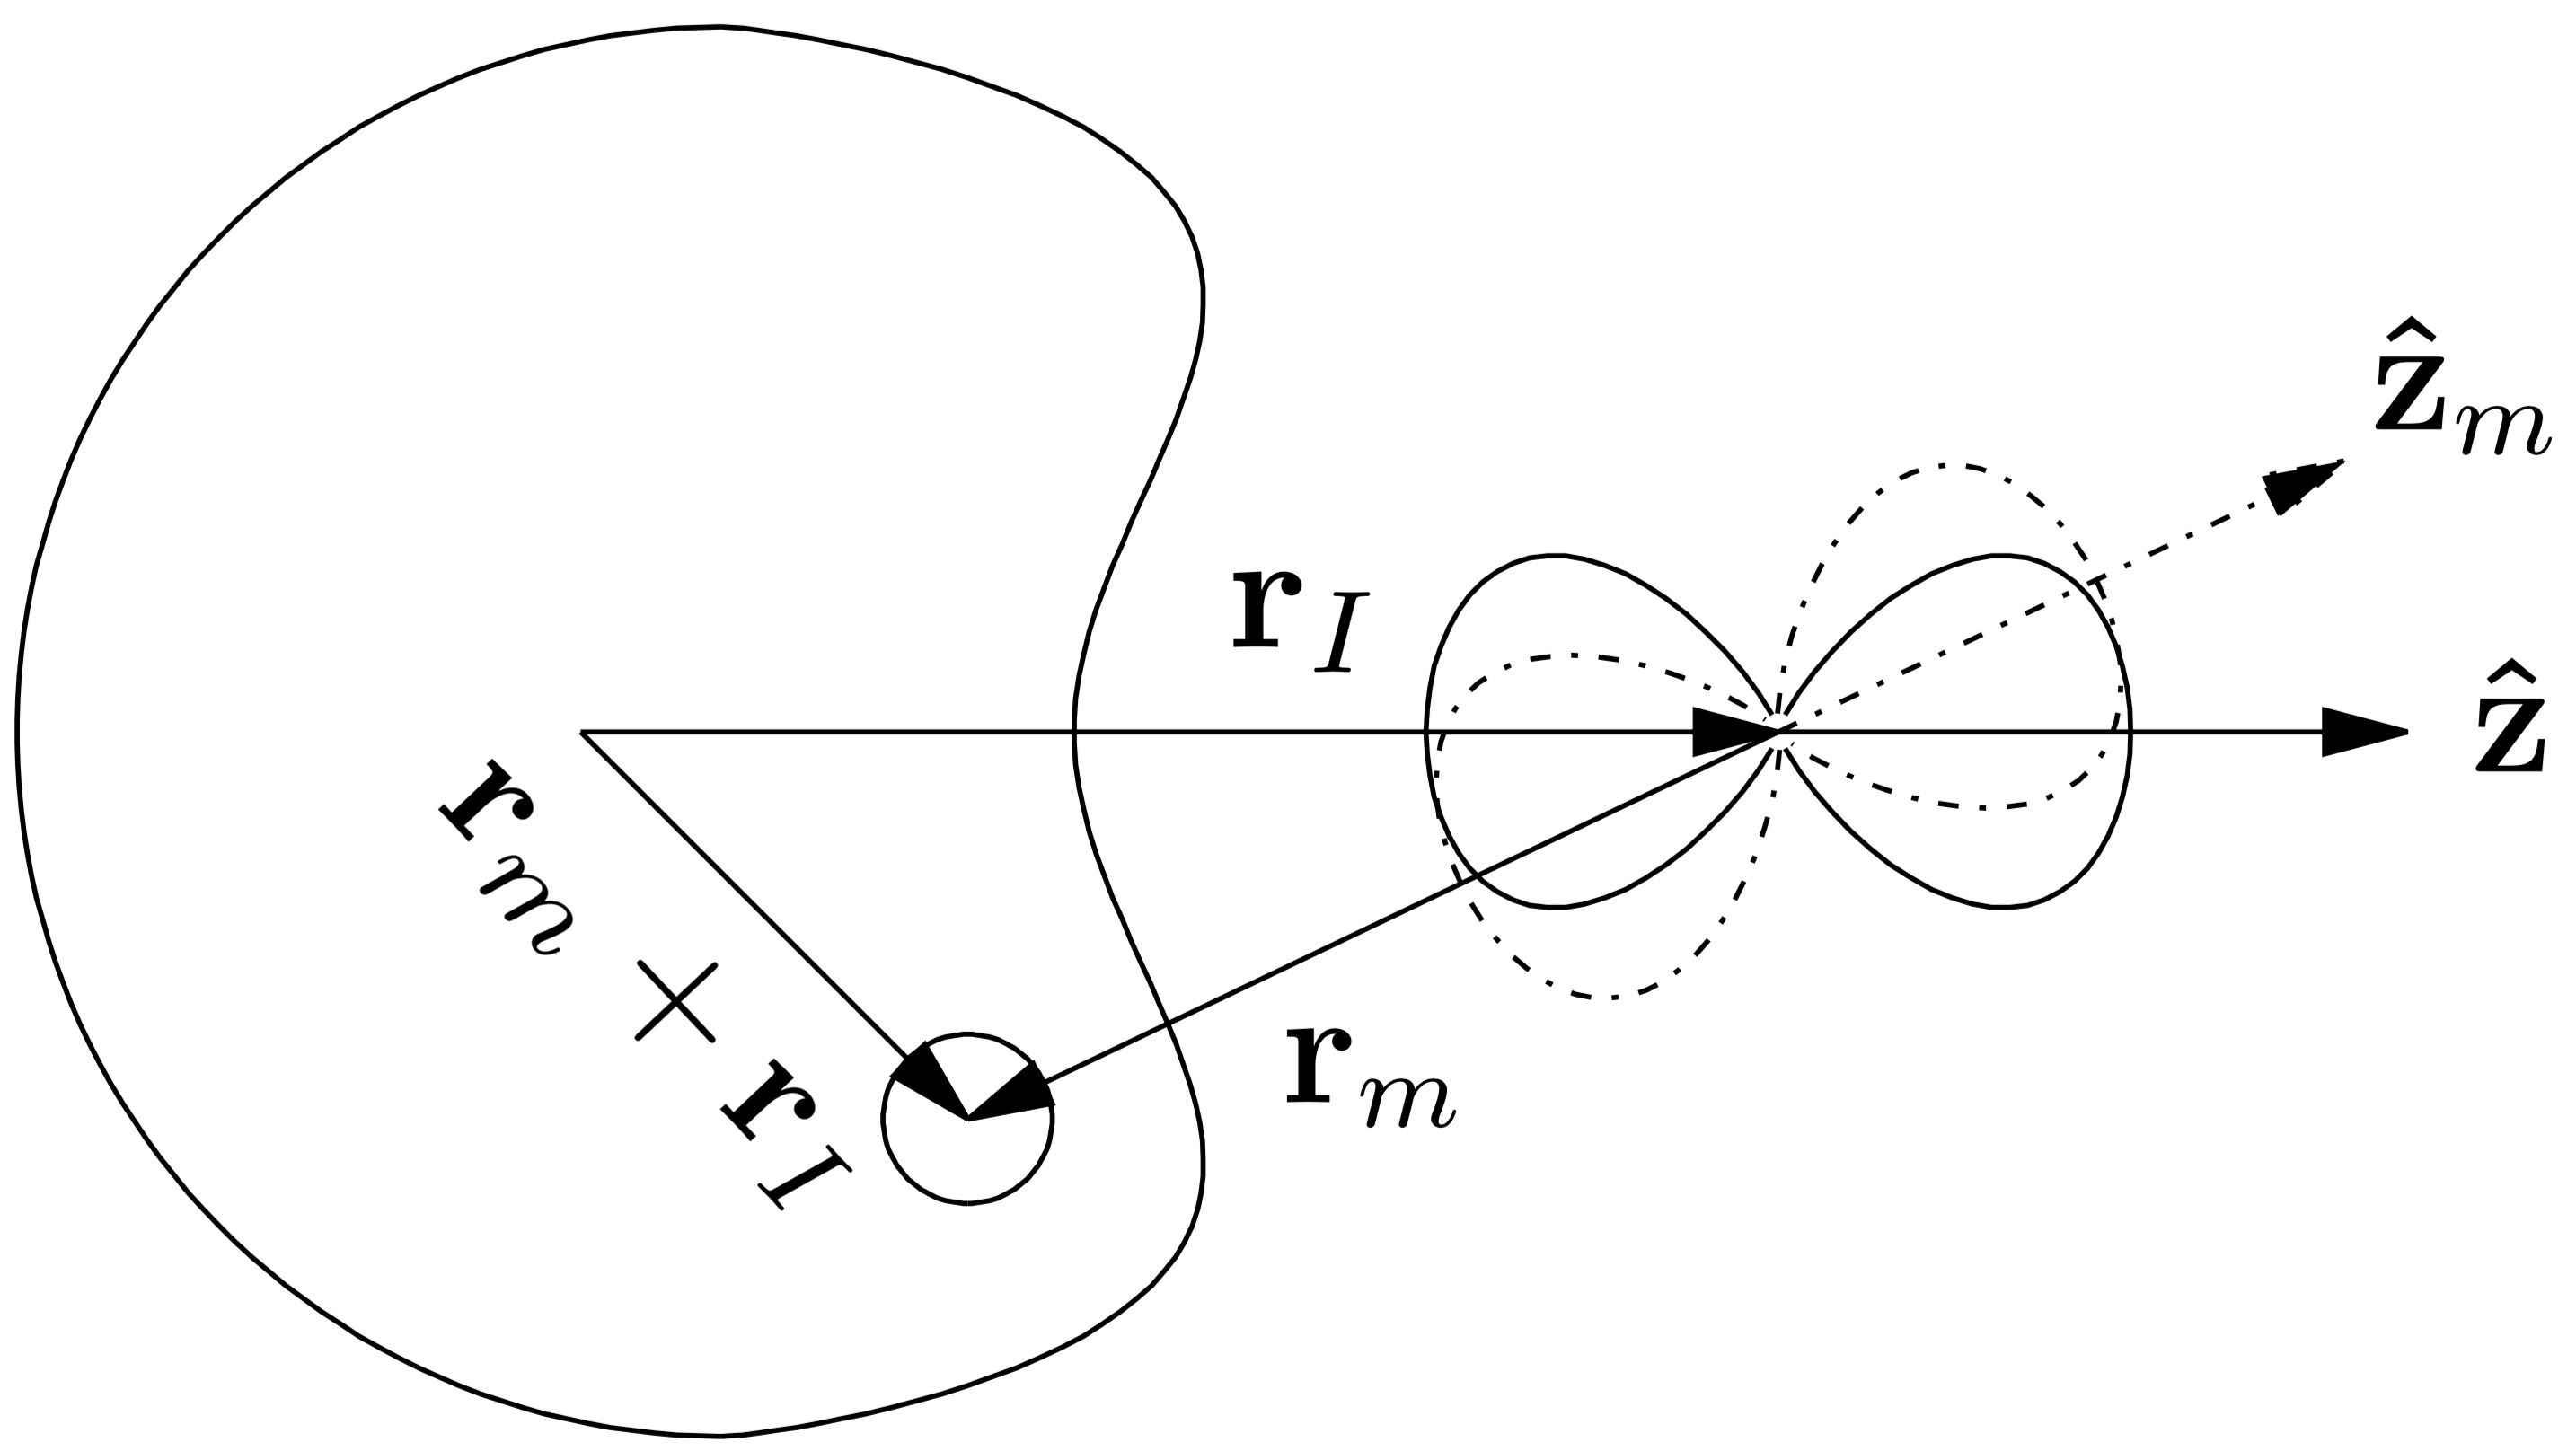
\includegraphics[width=0.75\textwidth]{dim-axes}
				\end{center}
				\caption{The set of axis defined in the DIM description (illustration courtesy of M. Martinez).}
				\label{fig:dim-axes}
			\end{figure}			
		
		\subsection{Including spin-orbit coupling}
			For the study of the alkali metal Rb in this work, the spin-orbit (SO) splitting of the energy levels is comparable to the splitting of the orbital angular momentum levels $L=0$ and $L=\pm 1$ due to the interaction with the helium. Therefore the spin-orbit interaction needs to be included in the total interaction Hamiltonian.\\
			
			The total Hamiltonian is given by the sum of the DIM-interaction and the SO-interaction $\mathcal{H} = \mathcal{U}^{DIM}+\mathcal{V}^{SO}$. The SO-matrix is defined
			\begin{align}
				\mathcal{V}^{SO}=\frac{1}{2}A_{\ell s}\qty(\vec{J}^2-\vec{L}^2-\vec{S}^2)
			\end{align}
			with $\vec{J}=\vec{L}+\vec{S}$. The coupling constant $A_{\ell s}$ is usually approximated by that of the free atom \cite{Jak97}. We can extend the DIM basis Eq. (\ref{eq:dim-basis}) to include the projection of the electron spin $s=\qty{\uparrow,\downarrow}$ corresponding to the quantum numbers $m_s=\qty{\frac{1}{2},-\frac{1}{2}}$:
			\begin{align}
				\ket{p_i,s}\in\qty\big{\,\ket{p_x,\uparrow}\!,\ket{p_x,\downarrow}\!,\ket{p_y,\uparrow}\!,\ket{p_y,\downarrow}\!,\ket{p_z,\uparrow}\!,\ket{p_z,\downarrow}}.
			\end{align}
			In this basis the $\mathcal{V}^{SO}$ is given by
			\begin{align}
				\mathcal{V}^{SO} = \frac{1}{2}A_{\ell s}\mqty*(0&0&-i&0&0&1\\0&0&0&i&-1&0\\i&0&0&0&0&-i\\0&-i&0&0&-i&0\\0&-1&0&i&0&0\\1&0&i&0&0&0)
			\end{align}
			Kramers' theorem states that the two-fold degeneracy of the levels originating from total half-integer spin cannot be broken by electrostatic interactions \cite{Nak01}. Therefore all the electronic eigenstates of $\mathcal{H}$ are doubly degenerate. Diagonalisation of $\mathcal{H}$ yields three doubly degenerate PECs between the impurity and surrounding helium.\\
			
			The dynamic evolution of the electronic excited state of the impurity is described by introducing an additional degree of freedom, a 6-component vector $\ket\lambda$, which describes the coefficients of the electronic state in the $\qty{\ket{p_i,s}}$ basis
			\begin{align}
				\ket{\lambda(t)} = \!\!\!\!\!\sum_{\substack{i=\{x,y,z\}\\s=\{\uparrow,\downarrow\}}}\!\!\!\!\! \lambda_{is}(t) \ket{p_i,s}
			\end{align}
			such that $\norm{\ip{\lambda}}^2=1$. The complete set of variables required to describe the
			system consists of the complex valued effective wave function for helium $\Psi(\mathbf{r}, t)$ with
			$\rho(\mathbf{r}, t) = |\Psi(\mathbf{r}, t)|^2$, the impurity position $\mathbf{r}_I(t)$, and the 6-dimensional complex vector to determine 
			its electronic wave function $|\lambda(t)\rangle$. The total energy of the impurity-$^4$He$_N$ complex after excitation to the $^2$P manifold is

			\begin{align}
				E[\Psi, \vec{r}_I, \lambda] &= \frac{\hbar^2}{2m}\int\!\abs{\grad \Psi}^2\diff{r}
				+ \int\!{\cal E}_c[\rho]\diff{r} \nonumber \\
				&+ \frac{p^2_I}{2 m_I}
				+ \int\!\rho(\vec{r})\,V_\lambda(\vec{r}-\vec{r}_I)\diff{r}
				+ \ev**{\mathcal{V}^{SO}}{\lambda}
			\end{align}
			where $V_\lambda$ is defined as
			\begin{align}
				V_\lambda(\vec{r}) \vcentcolon= \ev{\mathcal{V}^{DIM}}{\lambda} = \sum_{ijss'}\lambda^*_{is}V^{DIM}_{ijss'}(\vec{r})\lambda_{js'} 
			\end{align}
			and the components of the $6\times6$ matrix ${\mathcal V}^{DIM}$ given by
			\begin{equation}
				V^{DIM}_{ijss'}(\vec{r})=V^{DIM}_{ij}\delta_{ss'}=\qty{V_\Pi(r)\delta_{ij}+\qty\big[V_\Sigma(r)-V_\Pi(r)]\frac{r_i\,r_j}{\norm{\vec{r}_m}^2}}\delta_{ss'}
			\end{equation}
			Unlike for the static DFT case, the time evolution of the system is obtained by minimising the following action
			\begin{align}
				A[\Psi,\vec{r}_I,\lambda] = \int\!\bigg\{&E[\Psi,\vec{r}_I,\lambda] -i\hbar\int \!\Psi^*(\vec{r}) \pdv{t}\Psi(\vec{r})\dd{\vec{r}} \nonumber \\
				-&i\hbar\ev**{\pdv{t}}{\lambda} - \frac{1}{2} m_I \dot{\vec{r}}^2_I\bigg\}\dd{t}
			\end{align}
			Variation of the action $A$ with respect to $\qty\big{\Psi^*\!,\,\bra\lambda\!,\,\vec{r}_I}$ yields the following three coupled EL-equations
			\begin{align}
				i\hbar\pdv{t}\Psi &= \qty[-\frac{\hbar^2}{2m}\laplacian +\fdv{\mathcal{E}_c}{\rho(\mathbf{r})} + V_\lambda(\vec{r}-\vec{r}_I)]\Psi \nonumber \\
				i\hbar\pdv{t}\ket\lambda  &= \mathcal{H}\ket\lambda \nonumber \\
				m_I\ddot{\vec{r}}_I &= - \grad_{\vec{r}_I}\qty[\int\!\rho(\vec{r})\,V_\lambda(\vec{r}-\vec{r}_I)\dd{\vec{r}}] = -\int\!V_\lambda(\vec{r}-\vec{r}_I)\,\grad\rho(\vec{r})\dd{\vec{r}} \label{eq:dyn-el}
			\end{align}
			where the explicit time dependence of the variables is omitted for clarity. The second line of Eq. (\ref{eq:dyn-el}) is a $6\times 6$ matrix equation with the matrix elements of $\mathcal{H}$ given by
			\begin{align}
				H^{ijss'} = U^{DIM}_{ijss'}+V^{SO}_{ijss'} = \int\!\rho(\vec{r})\,V^{DIM}_{ijss'}(\vec{r}-\vec{r}_I)\dd{\vec{r}}+V^{SO}_{ijss'}
			\end{align}
			In the cases that SO-coupling can be neglected the 6-dimensional electronic state vector $\ket{\lambda}$ reduces to the 3-dimensional vector
			\begin{align}
				\ket{\lambda(t)} = \sum_{i=\{x,y,z\}} \lambda_{i}(t) \ket{p_i}
			\end{align}
			and the $6\times6$ matrix $\mathcal{H}$ reduces to a $3\times 3$ matrix with elements
			\begin{align}
				H^{ij} = U^{DIM}_{ij} = \int\!\rho(\vec{r})\,V^{DIM}_{ij}(\vec{r}-\vec{r}_I)\dd{\vec{r}}
			\end{align}\\
			
			For the technical details about how this method is implemented the interested reader is directed to [\ref{deft-guide}]. For the collection of Fortran code that has been used to obtain the results presented here see [\ref{bcn-tlse-hedft}]. For the manuel to use the code see [\ref{dft-manual}].
	

%		Introduce superfluids and their properties
%		* Frictionless capillary flow (no viscosity)
%		* Creeping up the walls seemingly defying gravity
%		* capillary fountain
%		* second sound: heat propagating in waves with a constant speed of "second sound" instead of diffusion
%		* Fluid is irrotational
%		* Vorticity is quantised
	 

%%		E, 1908, July 10:		Kamerlingh Onnes, Liquefaction of helium-4,\\
%%		E, 1932, July:			John C. McLennan, Observed liquid helium stops boiling
%below 2.2 K. \\
%%		E, 1932:				W.H. Keesom, A.P. Keesom, observed a singularity in the specific
%heat at T=2.2 K and called it the lambda-temperature, because of the shape of
%the temperature dependence of the specific heat resembling the greek letter
%lambda.\\
%%		E, 1935, February 16:	E.F. Burton, measured sharply decreasing viscosity
%below 2.2 K\\
%%		T, 1935, August 16:		F. London, found that the magnitude of the zero-point
%energy of helium-4 is comparable to the Van der Waals interaction. This
%explains why helium doesn't freeze at T=0 at normal atmospheric pressure.\\
%%		E, 1936, May:			W.H. Keesom, A.P. Keesom, Observed abnormally thermal
%conductance, calling it 'supra-heat-conducting'\\
%%		E, 1937, July 10:		J.F. Allen,R. Peierls, M. Zaki Uddin, also observed
%abnormally high heat conductance. This was the reason for the liquid not
%boiling below 2.2 K\\
%%		E, 1937, December 3:	Kapitza, observed that below lambda-point viscosity of
%helium II is roughly 1500 smaller than helium I at normal pressure. In analogy
%with superconductors he concluded that helium below lambda enters a special
%state which he called superfluid.	This was the first mention of the word
%superfluid.\\
%%		E, 1937, December 22:	Allen and Misener (1938) discovered that helium-ii is
%not just a liquid with a very low viscosity, but that its hydrodynamics
%required a completely new interpretation.\\
%%		E, 1938, 05 February: 	J.F. Allen, discovery of fountain effect\\
%%		T, 1938, April 9:		F. London, connects behaviour of helium-II to BEC (ideal
%BE-gas). calculated Tc=3.09 K and Cv(t) for ideal BE-gas and they were very
%close to helium-II. He concluded that it was difficult not to imagine a
%connection to BEC\\
%%		T, 1938, May 21:		L. Tisza, birth of the 2-fluid model\\
%
%					which leads to 
%
%	Explanation of superfluidity by 
%		* Fritz London (April 1938, London, F., Nature, 141, 643 (1938))
%l-transition in liquid helium is analogous to Bose-Einstein condensation
%%		* Laszlo Tisza (May 1938, L. Tisza, Nature, 141, 913 (1938)) extended
%London's proposal by invoking a two-fluid model for helium II, which could
%qualitatively explain the observed transport phenomena, including the fountain
%effect.
%%		* Lev Landau (1941) if the spectrum of elementary excitations satisfies
%suitable criteria, the flow of of the fluid cannot dissipate energy. Postulated
%"phonons" and "rotons" and the famous Landau criterion for superfluidity
%%		* Nikolay Nikolayevich Bogolyubov (Oct. 12, 1946. Publ. 1947): Derivation of
%the elementary excitation spectrum from a molecular theory, making no
%assumptions about the structure of the energy spectrum.


%	\section{Random stuff about BEC}
%	Most general (time-independent) many-body Hamiltonian
%	\begin{align}
%		H(\vec{r}_1,\ldots,\vec{r}_N, \vec{p}_1,\ldots,\vec{p}_N) =
%\sum_{i=1}^N
%\qty(-\frac{\hbar^2}{2m_i}\nabla_{\vec{r}_i}^2)+V(\vec{r}_i,\ldots,\vec{r}_N)
%	\end{align}
%	And accompanying Schrödinger equation to solve
%	\begin{align}
%		i\hbar\frac{\partial}{\partial t}\Psi(\vec{r}_1,\ldots,\vec{r}_N,t) =
%\qty[\sum_{i=1}^N
%\qty(-\frac{\hbar^2}{2m_i}\nabla_{\vec{r}_i}^2)+V(\vec{r}_i,\ldots,\vec{r}_N)
%]\Psi(\vec{r}_1,\ldots,\vec{r}_N,t)
%	\end{align}
%For a 2-body system and a potential that only depends on the relative
%coordinate $\vec{r}_1-\vec{r}_2$ the Hamiltonian reduces reduces to
%	\begin{align}
%		H(\vec{r}_1,\vec{r}_2) =
%-\qty(\frac{\hbar^2}{2m_1}\nabla_{\vec{r}_1}^2+\frac{\hbar^2}{2m_2}\nabla_{\vec
%{r}_2}^2)+V(\vec{r}_1-\vec{r}_2)
%	\end{align}
%By either introducing the relative coordinate $\vec{r}$ and the center-of-mass
%(CM) coordinate $\vec{R}$, or the relative momentum
%$\vec{p}$ and the total momentum $\vec{P}$, we can consider the motion of the
%CM itself ($\vec{R}$) and the motion relative to the CM
%	($\vec{r}$):
%	\begin{align}
%		H(\vec{R},\vec{r}) =
%-\qty(\frac{\hbar^2}{2M}\nabla_{\vec{R}}^2+\frac{\hbar^2}{2\mu}\nabla_{\vec{r}}
%^2)+V(\vec{r}),
%	\end{align}
%with $M=m_1+m_2$ and $\mu=\frac{m_1m_2}{m_1+m_2}$ (reduced mass of the system).
%	Schrödinger equation to solve
%	\begin{align}
%i\hbar\frac{\partial}{\partial t}\Psi(\vec{R},\vec{r},t) &=
%H(\vec{R},\vec{r})\Psi(\vec{R},\vec{r},t) \\
%&=
%\qty[-\qty(\frac{\hbar^2}{2M}\nabla_{\vec{R}}^2+\frac{\hbar^2}{2\mu}\nabla_
%{\vec{r}}^2)+V(\vec{r})]
%		\Psi(\vec{R},\vec{r},t) \label{eq:2b-se}
%	\end{align}
%	Assuming a separable solution and the given time-independence of the potential
%	\begin{align}
%\Psi(\vec{R},\vec{r},t) =
%\Phi(\vec{R})\psi(\vec{r})\mathrm{e}^{-i(E_{CM}+E)t/\hbar}
%	\end{align}
%and the 2-body Schrödinger equation (\ref{eq:2b-se}) separates into two
%mutually time-independent ODEs
%	\begin{align}
%-\frac{\hbar^2}{2M}\nabla_{\vec{R}}^2\Phi(\vec{R}) &= E_{CM}\Phi(\vec{R})
%\label{eq:se-fp}\\
%\qty[-\frac{\hbar^2}{2\mu}\nabla_{\vec{r}}^2 + V(\vec{r})]\psi(\vec{r}) &=
%E\psi(\vec{r}). \label{eq:se-muv}
%	\end{align}
%ODE (\ref{eq:se-fp}) describes the center of mass motion for a free particle
%with mass $M$ and energy
%$E_{CM}$. In one dimension the time-\emph{dependent normalizable} solution for
%such a particle,
%initially localized between $-a$ and $a$ is an integral over plane waves over
%all frequencies
%	\begin{align}
%\Phi(X,t) =
%\frac{1}{\pi}\sqrt{\frac{a}{2}}\int_{-\infty}^{+\infty}\!\mathrm{sinc}(ka)\,
%		\exp[i\qty(kX-\frac{\hbar k^2}{2M}t)]\,\mathrm{d}k.
%	\end{align}
%ODE (\ref{eq:se-muv}) describes the motion relative to the CM of a particle of
%reduced mass $\mu$ in a potential $V(\vec{r})$.
%	For hydrogen this is the Coulomb potential. Explicitly
%	\begin{align}
%\qty[-\frac{\hbar^2}{2\mu}\nabla_{\vec{r}}^2 -
%\frac{e^2}{(4\pi\varepsilon_0)r}]\psi(\vec{r}) &= E\psi(\vec{r}),
%	\end{align}
%where it is customary to switch to spherical polar coordinates and separate the
%solutions again
%	\begin{align}
%\psi(\vec{r}) \rightarrow \psi_{E,l,m}(r,\theta,\phi) =
%R_{E,l}(r)Y_{ml}(\theta,\phi),
%	\end{align}
%where $R_{E,l}$ is the radial wave function, fully determined by the energy $E$
%and the orbital angular momentum quantum
%number $l$ and $Y_{ml}$ are the spherical harmonics, fully determined by $l$
%and the magnetic quantum number $m$.
%	
%	\section{Helium-4, a 3-body system with 2 electrons}
%The unperturbed (omit electron-electron repulsion) ground state (as obtained by
%the `single particle model')
%	\begin{align}
%\psi_0^{(0)}(r_1,r_2) &= \psi_{1\mathrm{s}(r_1)}\psi_{1\mathrm{s}(r_2)} \otimes
%		\frac{1}{\sqrt{2}}\qty(\ket{\uparrow\downarrow}-\ket{\downarrow\uparrow}) \\ 
%&= \frac{8}{\pi}\exp[-2(r_1+r_2)] \otimes
%\frac{1}{\sqrt{2}}\qty(\ket{\uparrow\downarrow}-\ket{\downarrow\uparrow})
%	\end{align}
%Or in the `central field approximation' with effective nuclear charge
%$Z_e=1.70$
%	\begin{align}
%\psi_0(r_1,r_2) =
%\frac{4.913}{\pi}\exp[-1.70(r_1+r_2)]\otimes\frac{1}{\sqrt{2}}\qty(\ket
%{\uparrow\downarrow}-\ket{\downarrow\uparrow})
%	\end{align}

\end{document}